% \documentclass[paper=a4, fontsize=11pt]{scrartcl} % A4 paper and 11pt font size
\documentclass[a4paper,11pt]{book}
\usepackage[T1]{fontenc} % Use 8-bit encoding that has 256 glyphs
\usepackage[utf8]{inputenc}
\usepackage{fourier} % Use the Adobe Utopia font for the document - comment this line to return to the LaTeX default
\usepackage{listings} % para insertar código con formato similar al editor
\usepackage[spanish, es-tabla]{babel} % Selecciona el español para palabras introducidas automáticamente, p.ej. "septiembre" en la fecha y especifica que se use la palabra Tabla en vez de Cuadro
\usepackage{url} % ,href} %para incluir URLs e hipervínculos dentro del texto (aunque hay que instalar href)
\usepackage{graphics,graphicx, float} %para incluir imágenes y colocarlas
\usepackage[gen]{eurosym} %para incluir el símbolo del euro
\usepackage{cite} %para incluir citas del archivo <nombre>.bib
\usepackage{enumerate}
\usepackage{hyperref}
\usepackage{tabularx}
\usepackage{booktabs}
\usepackage{afterpage}
\usepackage{longtable}
\usepackage[stable]{footmisc}
\usepackage[table,xcdraw]{xcolor}
\usepackage[font=small,labelfont=bf,center]{caption}
\usepackage{subcaption}



% ********************************************************************
% Re-usable information
% ********************************************************************
\newcommand{\myTitle}{Técnicas de Deep Learning para el diagnóstico del Alzheimer\xspace}
\newcommand{\myTitleEn}{Deep Learning techniques for Alzheimer's disease diagnosis\xspace}
\newcommand{\myDegree}{Grado en Ingeniería Informática\xspace}
\newcommand{\myName}{Raquel Molina Reche\xspace}
\newcommand{\myProf}{Rosa María Rodríguez Sánchez\xspace}
\newcommand{\myFaculty}{Escuela Técnica Superior de Ingenierías Informática y de Telecomunicación\xspace}
\newcommand{\myFacultyShort}{E.T.S. de Ingenierías Informática y de Telecomunicación\xspace}
\newcommand{\myDepartment}{Departamento de Ciencias de la Computación e Inteligencia Artificial\xspace}
\newcommand{\myProject}{Trabajo Fin de Grado\xspace}
\newcommand{\myUni}{\protect{Universidad de Granada}\xspace}
\newcommand{\myLocation}{Granada\xspace}
\newcommand{\myTime}{\today\xspace}
\newcommand{\myVersion}{Version 0.1\xspace}


\hypersetup{
    colorlinks=true,	% false: boxed links; true: colored links
    linkcolor=black,	% color of internal links
    urlcolor=cyan		% color of external links
}


\renewcommand{\familydefault}{\sfdefault}
\usepackage{fancyhdr} % Custom headers and footers
\pagestyle{fancyplain} % Makes all pages in the document conform to the custom headers and footers
\fancyhf{} % clear existing header/footer entries
% HEADER
\setlength{\headheight}{13.6pt} % Customize the height of the header
\fancyhead[L]{} % Empty left header
\fancyhead[C]{} % Empty center header
\fancyhead[R]{} % Empty right header
\fancyhead[LO]{\leftmark}
\fancyhead[RE]{\rightmark}
\fancyhead[RO,LE]{\thepage}
\renewcommand{\chaptermark}[1]{\markboth{#1}{}}
\renewcommand{\sectionmark}[1]{\markright{\thesection. #1}}
% FOOOTER
\renewcommand{\footrulewidth}{0pt} % Remove footer underlines
\fancyfoot[L]{} % Empty left footer
\fancyfoot[C]{} % Empty center footer

\fancypagestyle{plain}{%
    \fancyhf{}% clear all header and footer fields
    \fancyfoot[C]{\thepage} % except the center
    \renewcommand{\headrulewidth}{0pt}%
    \renewcommand{\footrulewidth}{0pt}%
}

\fancypagestyle{coverpage}{%
    \fancyhf{}% clear all header and footer fields
    \fancyhead[L]{\myProject} % except the center
%    \renewcommand{\headrulewidth}{0pt}%
    \renewcommand{\footrulewidth}{0pt}%
}


\usepackage{titlesec, blindtext, color}
\newcommand{\hsp}{\hspace{20pt}}
\titleformat{\chapter}[hang]{\Huge\bfseries}{\thechapter\hsp{|}\hsp}{0pt}{\Huge\bfseries}
\setcounter{secnumdepth}{3} % Turn off/on section numbers (0=no numbers, 1=numbers in sections, 2=numbers in subsections ...)
\setcounter{tocdepth}{3}
%\usepackage[Lenny]{fncychap}


\newcommand{\HRule}{\rule{\linewidth}{0.5mm}}
\newcommand{\bigrule}{\titlerule[0.5mm]}


%Definimos los tipos teorema, ejemplo y definición podremos usar estos tipos
%simplemente poniendo \begin{teorema} \end{teorema} ...
\newtheorem{teorema}{Teorema}[chapter]
\newtheorem{ejemplo}{Ejemplo}[chapter]
\newtheorem{definicion}{Definición}[chapter]

\definecolor{gray97}{gray}{.97}
\definecolor{gray75}{gray}{.75}
\definecolor{gray45}{gray}{.45}
\definecolor{gray30}{gray}{.94}

\lstset{ frame=Ltb,
    framerule=0.5pt,
    aboveskip=0.5cm,
    framextopmargin=3pt,
    framexbottommargin=3pt,
    framexleftmargin=0.1cm,
    framesep=0pt,
    rulesep=.4pt,
    backgroundcolor=\color{gray97},
    rulesepcolor=\color{black},
%
    stringstyle=\ttfamily,
    showstringspaces = false,
    basicstyle=\scriptsize\ttfamily,
    commentstyle=\color{gray45},
    keywordstyle=\bfseries,
%
    numbers=left,
    numbersep=6pt,
    numberstyle=\tiny,
    numberfirstline = false,
    breaklines=true,
}

% minimizar fragmentado de listados
\lstnewenvironment{listing}[1][]
{\lstset{#1}\pagebreak[0]}{\pagebreak[0]}

\lstdefinestyle{CodigoC}
{
    basicstyle=\scriptsize,
    frame=single,
    language=C,
    numbers=left
}
\lstdefinestyle{CodigoC++}
{
    basicstyle=\small,
    frame=single,
    backgroundcolor=\color{gray30},
    language=C++,
    numbers=left
}


\lstdefinestyle{Consola}
{
    basicstyle=\scriptsize\textbf{\ttfamily},
    backgroundcolor=\color{gray30},
    frame=single,
    numbers=none
}

%Para conseguir que en las páginas en blanco no ponga cabecerass
\makeatletter
\renewcommand{\clearpage}{%
    \ifvmode
    \ifnum \@dbltopnum =\m@ne\ifdim \pagetotal <\topskip
    \hbox{}
    \fi
    \fi
    \fi
    \newpage
    \thispagestyle{empty}
    \write\m@ne{}
    \vbox{}
    \penalty -\@Mi
}
\makeatother

\usepackage{glossaries}
\newglossaryentry{IA}
{ name=IA, description={Inteligencia Artificial.}}

\newglossaryentry{EA}
{ name=EA, description={Enfermedad del Alzheimer.}}

\newglossaryentry{MRI}
{ name=MRI, description={Imagen por Resonancia Magnética. Magnetic Resonance Imaging.}}

\newglossaryentry{PET}
{ name=PET, description={Tomografía por emisión de positrones. Positron Emission Tomography.}}

\newglossaryentry{DL}
{ name= DL, description={Aprendizaje Profundo.Deep Learning.}}

\newglossaryentry{ML}
{ name=ML, description={Aprendizaje Automático.Machine Learning.}}

\newglossaryentry{TFG}
{ name=TFG, description={Trabajo de Fin de Grado.}}

\newglossaryentry{HU}
{ name=HU, description={Historias de Usuario.}}

\newglossaryentry{ROI}
{ name=ROI, description={Regiones De Interés. Region of interest.}}

\newglossaryentry{CNN}
{ name=CNN, description={Redes Neuronales Convolucionales. Convolutional Neural Network.}}

\newglossaryentry{TL}
{ name=TL, description={Aprendizaje Por Transferencia. Transfer Learning.}}

\newglossaryentry{CN}
{ name=CN, description={Cognitivamente Normal. Cognitively Normal.}}

\newglossaryentry{MCI}
{ name=MCI, description={Deterioro Cognitivo Leve. Mild cognitive impairment.}}

\newglossaryentry{AD}
{ name=AD, description={Enfermedad de Alzheimer. Alzheimer's Disease.}}



\makenoidxglossaries

\begin{document}

    % Plantilla portada UGR
    \begin{titlepage}


\newlength{\centeroffset}
\setlength{\centeroffset}{-0.5\oddsidemargin}
\addtolength{\centeroffset}{0.5\evensidemargin}
\thispagestyle{empty}

\noindent\hspace*{\centeroffset}\begin{minipage}{\textwidth}

\centering

\includegraphics[width=0.9\textwidth]{logos/logo_ugr.jpg}\\[1.4cm]

\textsc{ \Large TRABAJO FIN DE GRADO\\[0.2cm]}
\textsc{ GRADO EN INGENIERÍA INFORMÁTICA}\\[1cm]
% Upper part of the page
% 
% Title
{\Huge\bfseries Técnicas de Deep Learning para el diagnóstico del Alzheimer\\}
\noindent\rule[-1ex]{\textwidth}{3pt}\\[3.5ex]
%{\large\bfseries Subtitulo del Proyecto}
\end{minipage}


\vspace{2.5cm}

\noindent\hspace*{\centeroffset}\begin{minipage}{\textwidth}
\thispagestyle{empty}
\centering

\textbf{Autor}\\ {Raquel Molina Reche}\\[2.5ex]
\textbf{Director}\\ {Rosa María Rodriguez Sánchez}\\[2cm]

\includegraphics[width=0.3\textwidth]{logos/etsiit_logo.png}\\[0.1cm]
\textsc{Escuela Técnica Superior de Ingenierías Informática y de Telecomunicación}\\
\textsc{---}\\
Granada, Junio de 2022


\end{minipage}
\end{titlepage}




    % Plantilla prefacio UGR
    \thispagestyle{empty}

\begin{center}
{\large\bfseries \myTitle}\\
\end{center}
\begin{center}
       \myName\\
\end{center}

\vspace{0.7cm}
\noindent{\textbf{Palabras clave}: palabra\_clave1, palabra\_clave2, palabra\_clave3, ......}\\

\vspace{0.7cm}
\noindent{\textbf{Resumen}}\\

Poner aquí el resumen.
\cleardoublepage
\thispagestyle{empty}


\begin{center}
{\large\bfseries \myTitleEn}\\
\end{center}
\begin{center}
       \myName\\
\end{center}

\vspace{0.7cm}
\noindent{\textbf{Keywords}: Keyword1, Keyword2, Keyword3, ....}\\

\vspace{0.7cm}
\noindent{\textbf{Abstract}}\\

Write here the abstract in English.

%\cleardoublepage
%\thispagestyle{empty}
%
%\noindent\rule[-1ex]{\textwidth}{2pt}\\[4.5ex]
%
%Yo, \textbf{Raquel Molina Reche}, alumna de la titulación Ingeniería Informática de la \textbf{Escuela Técnica Superior
%de Ingenierías Informática y de Telecomunicación de la Universidad de Granada}, con DNI 49627634M, autorizo la
%ubicación de la siguiente copia de mi Trabajo Fin de Grado en la biblioteca del centro para que pueda ser
%consultada por las personas que lo deseen.
%
%\vspace{6cm}
%
%\noindent Fdo: Raquel Molina Reche
%
%\vspace{2cm}
%
%\begin{flushright}
%Granada a X de mes de 201 .
%\end{flushright}


\cleardoublepage
\thispagestyle{empty}

\noindent\rule[-1ex]{\textwidth}{2pt}\\[4.5ex]

Dª. \textbf{\myProf}, Profesora del \myDepartment de la \myUni.

\vspace{0.5cm}

\textbf{Informa:}

\vspace{0.5cm}

Que el presente trabajo, titulado \textit{\textbf{\myTitle}},
ha sido realizado bajo su supervisión por \textbf{\myName}, y autorizo la defensa de dicho trabajo ante el tribunal
que corresponda.

\vspace{0.5cm}

Y para que conste, expido y firmo el presente informe en \myLocation a \myTime.

\vspace{1cm}

\textbf{La directora:}

\vspace{5cm}

\noindent \textbf{\myProf}

\chapter*{Agradecimientos}
\thispagestyle{empty}

       \vspace{1cm}


Poner aquí agradecimientos...



    \frontmatter

    % Índice de contenidos
    \newpage
    \tableofcontents

    % Índice de imágenes y tablas
    \newpage
    \listoffigures

    \newpage
    \listoftables

    \printnoidxglossaries\addcontentsline{toc}{chapter}{Glosario}

    \mainmatter
    \setlength{\parskip}{5pt}

    \chapter{Introducción}\label{ch:introduccion}

Este proyecto está publicado bajo la licencia GNU General Public License v3~\cite{gplv3}.
Se puede acceder a través de GitHub en este \href{https://github.com/raquelmolinare/TFG}{enlace}.


\section{Motivación y contexto}\label{sec:motivacion-y-contexto}
A día de hoy, gracias a los avances en ciencias de la computación, la inteligencia artificial (en adelante \Gls{IA}) se está
convirtiendo en una parte fundamental de la atención médica actual.
Algoritmos y aplicaciones impulsadas por IA se usan en el día a día para ayudar a los profesionales en entornos clínicos
y en el ámbito de la investigación.

Según la Confederación Española de Alzheimer (CEAFA)~\cite{ceafa} la \textbf{Enfermedad del Alzheimer} (en adelante \Gls{EA})
es una enfermedad neurodegenerativa que afecta a aproximadamente 1.200.000 personas en España y a más de 50 millones de
personas en el mundo según un artículo de la Universitat Oberta de Catalunya (UOC)~\cite{uoc}.
Es una enfermedad progresiva, o lo que es lo mismo, que empeora con el tiempo y para la que no existe una cura, solo
la posibilidad de aplicar tratamientos que ralenticen su avance.
Para que estos tratamientos no resulten perjudiciales para la salud del paciente deben realizarse en las primeras etapas
de la enfermedad.
Por ello un diagnóstico temprano puede ser determinante para el paciente, pero, en la mayoría de casos, detectar esta
enfermedad en las primeras fases de la misma es una tarea muy compleja.

Investigaciones previas han concluido que las primeras lesiones cerebrales pueden aparecer incluso 20 años antes de que
aparezcan los primeros síntomas del Alzheimer~\cite{ceafa}.
De hecho una de las evaluaciones médicas para la detección de la enfermedad se basa en el diagnóstico por imágenes
cerebrales mediante la realización de un examen imagenológico, que puede incluir técnicas como: Imagen por Resonancia
Magnética (en adelante MRI), Tomografía Computarizada o Tomografía por emisión de positrones (en adelante \Gls{PET}).

A día de hoy el aprendizaje profundo o deep learning (en adelante \Gls{DL})  ha levantado mucho interés en el mundo de la
medicina.
El Deep learning es un subconjunto del machine learning (en adelante \Gls{ML}) en IA, que simula el comportamiento del cerebro
humano en el procesamiento de datos y el reconocimiento de patrones para resolver problemas complejos de toma de
decisiones.

Es por esto que el uso de DL puede ayudar a un diagnóstico temprano, ya que estos sistemas pueden ser utilizados para la
detección de anomalías en imágenes médicas donde destaca la rapidez de la detección, sirviendo como herramienta de
prevención y seguimiento de la enfermedad.

También cabe destacar que la enfermedad del Alzheimer presenta diferentes fases y la velocidad a la que avanza la
enfermedad por las diferentes fases varía, por lo que es más difícil realizar predicciones a largo plazo.
Se usan escalas con distinto número de fases:
\begin{itemize}
    \item \textbf{La escala de deterioro global (GDS)}~\cite{gds} se divide en siete fases que dependen del valor del
    deterioro cognitivo y más común utilizarla para escalar la demencia senil.
    Sus fases son: ausencia de alteración cognitiva, disminución cognitiva muy leve, defecto cognitivo leve, defecto
    cognitivo moderado, defecto cognitivo moderado-grave, defecto cognitivo grave y defecto cognitivo muy grave.
    \item \textbf{La escala de clasificación de la demencia clínica (CDR)}~\cite{cdr} se divide en cinco fases, es la más
    utilizada en el área de investigación y evalúa diferentes parámetros como la memoria, la orientación, la resolución
    de problemas, el juicio, etc.
    Sus fases son: Cognitivamente sano (CDR 0), demencia cuestionable (CDR 0.5), demencia leve (CDR 1), demencia
    moderada (CDR 2) y demencia grave (CDR 3).
    \item \textbf{La escala de clasificación común}~\cite{alz-org-etapas} solo tiene en cuenta tres fases, es la más
    usada en la comunicación médico-familia, ya que es la más sencilla de comprender.
    Las fases que tiene en cuenta son: Enfermedad de Alzheimer leve (etapa temprana), enfermedad de Alzheimer moderada
    (etapa media) y enfermedad de Alzheimer grave (etapa final).\\
\end{itemize}

A día de hoy, realizar estudios en esta área significa conseguir grandes avances en el mundo de la medicina y del
diagnóstico del Alzheimer, ayudando a mejorar la vida de los pacientes y las familias.
Por lo tanto, la motivación de este trabajo se centra en el estudio del uso de técnicas de Deep Learning para el
diagnóstico del Alzheimer a partir de imágenes cerebrales.




\section{Objetivos}\label{sec:objetivos}
El objetivo general de este proyecto es identificar qué plano cerebral ofrece mejor rendimiento para el diagnóstico del
Alzheimer mediante el uso de técnicas de Deep Learning a partir de Imágenes por Resonancia Magnética y facilitar su uso
en una aplicación real.

Este estudio se puede dividir en los siguientes objetivos específicos:
\begin{itemize}
    \item Conocer los conceptos teóricos del cuadro clínico, fases y diagnóstico de la EA.
    \item Estudiar las herramientas de DL y de procesamiento de imágenes más usadas actualmente para el diagnóstico del
    Alzheimer.
    \item Realizar un análisis y tratamiento de biomarcadores de Imagen por Resonancia Magnética.
    \item Analizar y seleccionar la arquitectura del sistema de DL para la resolución del problema.
    \item Evaluar el rendimiento que ofrecen los distintos planos cerebrales: axial, coronal y sagital al aplicar la
    técnica escogida.
    \item Desarrollar una aplicación web como ejemplo de uso real del sistema de aprendizaje profundo generado para
    facilitar la labor de los profesionales de entornos clínicos en el diagnóstico de la EA.\\
\end{itemize}




\section{Metodología, herramientas y obstáculos}\label{sec:metodologia-herramientas-y-obstaculos}
Una vez definidos los objetivos del problema a resolver, se explica a continuación la metodología y herramientas
implicadas en el desarrollo del proyecto y los posibles problemas que pueden surgir.

\subsection{Metodología}\label{subsec:metodologia}
Para conseguir los objetivos del  proyecto se ha seguido un desarrollo ágil en el que se han marcado 2 enfoques
principales:
\begin{itemize}
    \item El Trabajo de Fin de Grado (en adelante \Gls{TFG}) como proyecto, que engloba la construcción del sistema de DL, y
    en el que el cliente es el usuario lector de este trabajo.
    \item La aplicación web como proyecto con profesionales de entornos clínicos como clientes.\\
\end{itemize}

El desarrollo ágil es una metodología de trabajo cuyo objetivo principal es adaptarse a los cambios o necesidades
temporales de un proyecto y está basada en el desarrollo iterativo e incremental.
Mediante esta metodología se puede dividir el proyecto en tareas agrupadas en pequeñas etapas y que mediante su
finalización van añadiendo valor al producto final.

Los métodos ágiles de desarrollo de software usados a día de hoy se fundamentan en el trabajo en equipo, puesto que este
proyecto no está realizado por un equipo, si no que se elabora por una sola persona, se ha decidido seguir una
metodología de desarrollo ágil personalizada basada en los principios de las metodologías ágiles desarrollo de
software comunes:
\begin{itemize}
    \item Perseguir la satisfacción del cliente.
    En este caso del usuario lector y de profesionales de entornos clínicos.
    \item División del trabajo en fases temporales productivas compuestas por tareas simples.
    \item Medición del progreso.
    \item Adaptación a cambios.\\
\end{itemize}

\subsection{Herramientas}\label{subsec:herramientas}
Las herramientas empleadas para conseguir los objetivos del proyecto mediante la metodología explicada anteriormente se
detallan en esta sección.

Para llevar a cabo la medición del progreso se hace uso \textit{GIT} como sistema de control de versiones y
\textit{GitHub} como forja para alojar el proyecto, no solo por ser una herramienta considerablemente conocida y
utilizada en el día a día sin no también porque nos ofrece un amplio abanico de herramientas para construir software
seguro integradas en la propia plataforma como son los \textit{tableros Kanban} o Integración Continua mediante
\textit{GitHub Actions} entre otros.

Para este trabajo se han creado dos proyectos o \textit{tableros Kanban} en \textit{GitHub}, uno para la medición del
progreso del propio TFG y otro para la aplicación web a desarrollar, tal y como se comenta en el apartado anterior.
También se han definido un conjunto de \textit{milestones} para marcar puntos específicos del proyecto que reúnen diversas
\textit{issues}, las cuales tras completarse marcan la finalización del \textit{milestone} al que pertenecen.


\subsubsection{Milestones}
Los \textit{milestones} en este trabajo han señalado productos mínimos viables, de tal manera que completar todos los
\textit{milestones} da lugar a la finalización del proyecto y además se pretende que conforme se vayan completando
\textit{milestones} se vayan concluyendo los distintos objetivos que engloban este proyecto.
Los \textit{milestones} creados han sido los siguientes:
\begin{itemize}
    \item  \textbf{1. Base e introducción}: Preparación del entorno y sistema de trabajo y abarca la parte inicial de la
    memoria y de investigación del proyecto.
    \item \textbf{2. Análisis y Desarrollo experimental}: Desarrollo de un sistema de aprendizaje profundo a partir de
    Imágenes por Resonancia Magnética capaz de predecir el grado de Alzheimer presente en la imagen.
    Atendiendo a la literatura actual recopilada en el primer milestone.
    \item \textbf{3. Desarrollo de la aplicación web}: Construir una app que facilite el diagnóstico de la EA integrando el
    sistema de aprendizaje profundo implementado.
    \item \textbf{4. Conclusión}: Incluye la conclusión final de todo el proyecto y la finalización de los elementos
    introductorios.\\
\end{itemize}

\subsubsection{Historias de usuario}
Dentro de las \textit{issues} de \textit{GitHub} se ha diferenciado entre Historias de Usuario (en adelante \Gls{HU}) o
tareas.
A parte de diferenciarse en la nomenclatura se ha hecho uso de etiquetas para clasificar las \textit{issues}, las cuales
han sido:

\begin{itemize}
    \item \textit{user story}: para marcar HU.
    \item \textit{task}: para marcar tareas.
    \item \textit{research}: para marcar tareas relacionadas con investigación.
    \item \textit{documentation}: para marcar tareas relacionadas con documentación.
    \item \textit{development}: para marcar tareas relacionadas con desarrollo. \\
\end{itemize}

Las HUs  han marcado los objetivos y expresado las necesidades de los usuarios de nuestro proyecto desde su punto de
vista, dando lugar a las siguientes:
\begin{itemize}
    \item \textbf{Como lector quiero poder conocer la envergadura del proyecto de manera sencilla y ordenada a partir de la
    memoria}: Forma parte del concepto del proyecto como TFG. Como criterio de aceptación la memoria debe ser ordenada,
    clara y concisa de forma que se entienda el trabajo.
    \item \textbf{Como lector quiero conocer qué plano cerebral ofrece mejor rendimiento para el diagnóstico de la Enfermedad de
    Alzheimer mediante técnicas de aprendizaje profundo}: Engloba el desarrollo experimental del sistema de DL para el
    diagnóstico de la EA. Como criterio de aceptación  se debe llegar a una conclusión final sobre el plano que ofrece
    mayor rendimiento.
    \item \textbf{Como profesional de entornos clínicos quiero poder conocer el grado de Enfermedad de Alzheimer en una
    resonancia magnética de manera sencilla}:  Engloba el desarrollo de la aplicación web y se detalla más detenidamente
    en el capítulo~\ref{ch:aplicacion-web-para-el-diagnostico-del-alzheimer-mediante-mri}. \\
\end{itemize}

\begin{figure}[H]
    \centering
    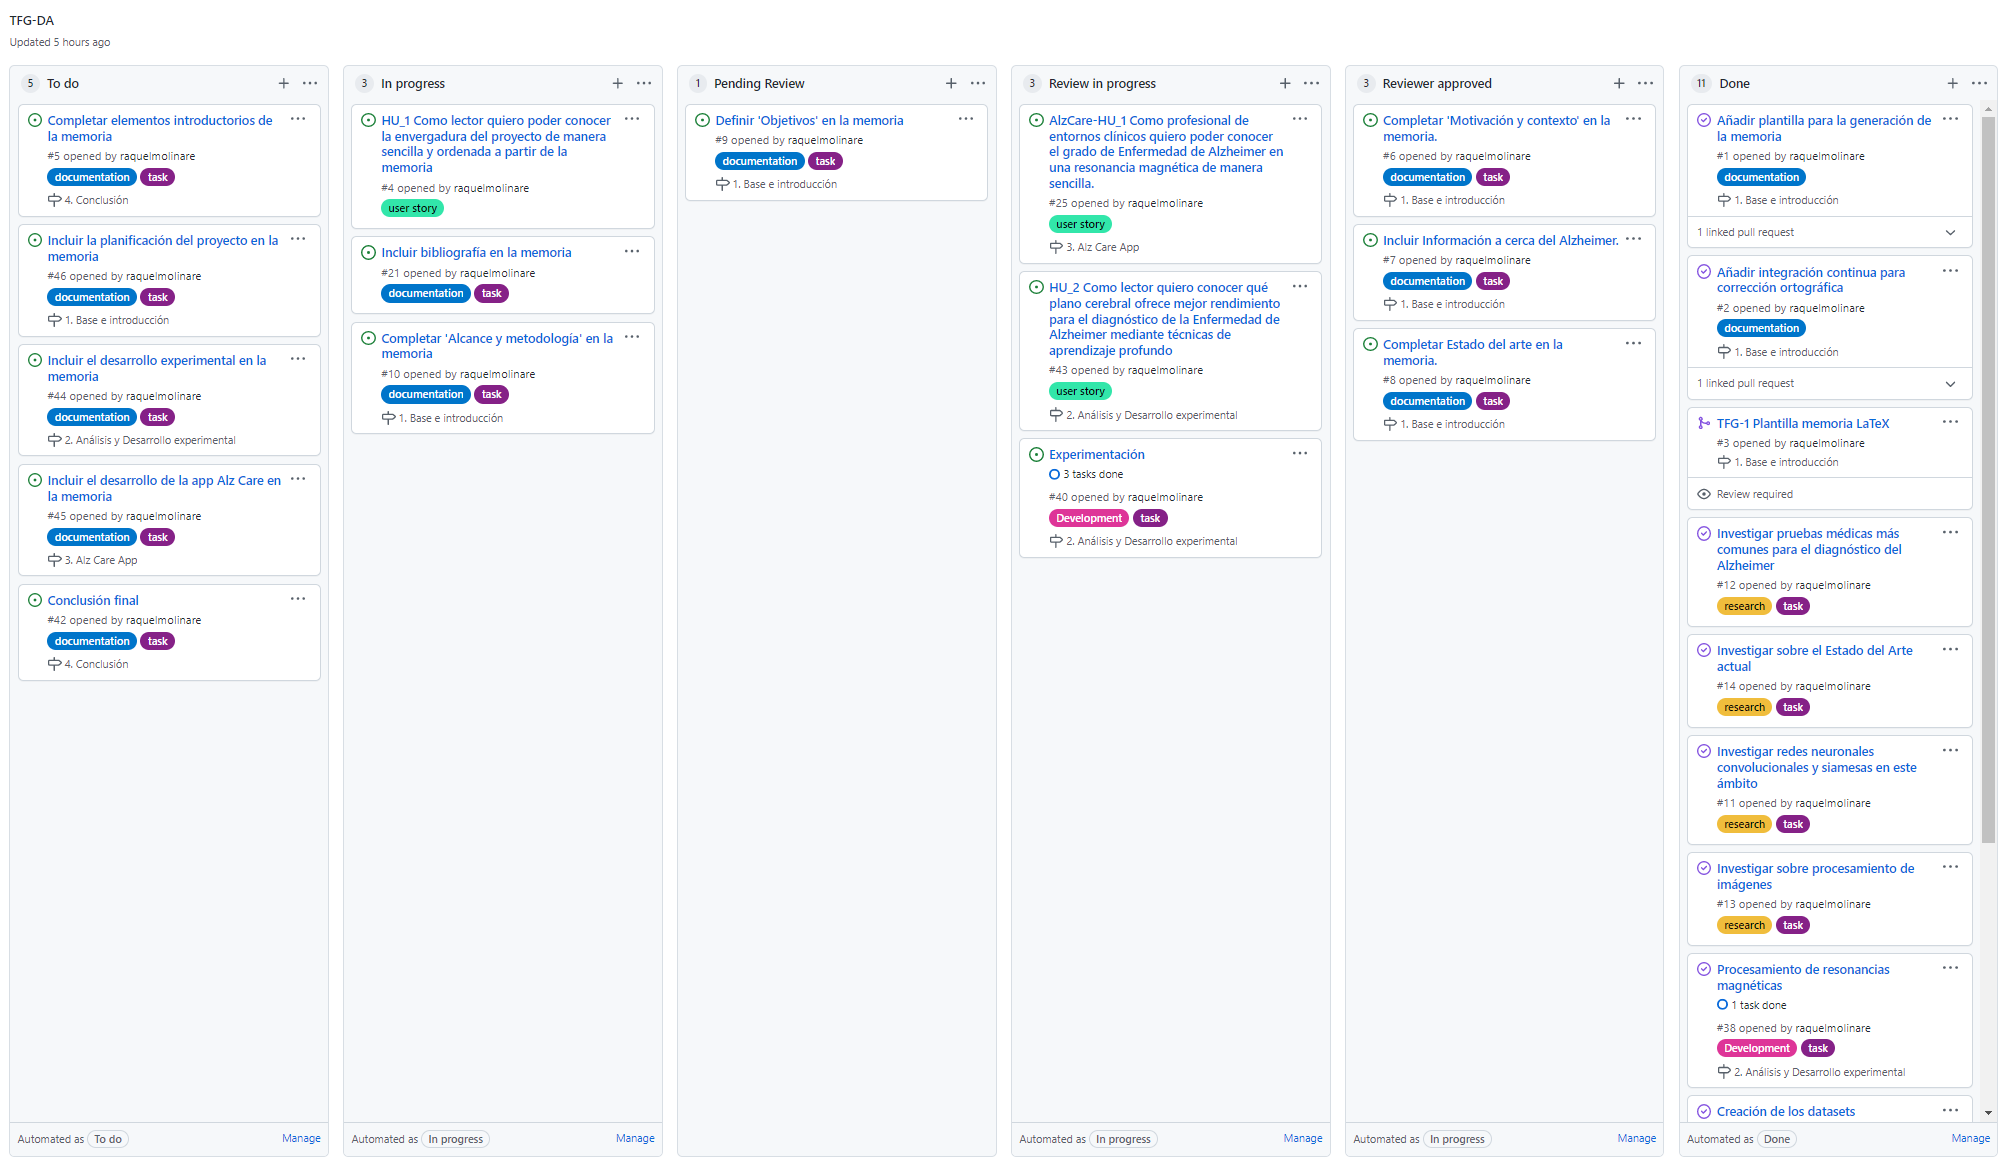
\includegraphics[width=\textwidth]{./imgs/tablero-github}
    \caption{Tablero Kanban del TFG desde GitHub}
    \label{fig:tablero-kanban-github}
\end{figure}

\subsubsection{Integración continua}
La Integración Continua es una práctica de desarrollo software en la que se ejecutan pruebas automáticas sobre nuevos
cambios realizados en el proyecto y que permite identificar errores presentes de manera inmediata.

Mediante \textit{GitHub Actions} se han automatizado y personalizado los flujos de trabajo en el repositorio del proyecto
incluyéndose:
\begin{itemize}
    \item Un corrector gramatical que realiza una revisión de la ortografía cada vez que se incluyen nuevos cambios en
    la memoria.
    \item Dos pipelines para el código de la aplicación que se detallan en la sección~\ref{sec:implementacion}.\\
\end{itemize}

Además se ha restringido que la fusión de ramas no se pueda realizar si no se han pasado los pipelines con éxito.

Todo lo que se ha comentado en esta sección sobre \textit{GitHub} se puede ver en el repositorio del
\href{https://github.com/raquelmolinare/TFG}{TFG}.

\subsection{Obstáculos}\label{subsec:obstaculos}
Si bien los objetivos están claramente definidos, es probable que durante la realización de este trabajo aparezcan 
obstáculos y por eso, tal como se ha indicado en el apartado~\ref{subsec:metodologia}, se ha optado por seguir un
desarrollo ágil preparado a cambios por los problemas o modificaciones que puedan surgir.
En este apartado se prevén los posibles problemas que pueden surgir durante el desarrollo del proyecto:

\subsubsection{Conjuntos de datos}
Los conjuntos de biomarcadores disponibles del seguimiento de la EA son muy reducidos, lo que puede suponer una
limitación importante en el desarrollo experimental del sistema de aprendizaje profundo, dando lugar a un sobreajuste.

\subsubsection{Requerimiento computacional}
Las técnicas de DL requieren de un elevado coste computacional el cual varía dependiendo de la arquitectura utilizada.
Por lo que puede ser necesario descartar arquitecturas de tipo 3D, que frente a las de tipo 2D tienen un notablemente
mayor requerimiento computacional.



    \chapter{Planificación del proyecto}\label{ch:planificacion}
En esta sección se incluyen los aspectos relativos a la planificación del proyecto.
Incluyendo un test de viabilidad, planificación temporal, diagrama de Gantt y el presupuesto asociado al
trabajo.


\section{Test de viabilidad}\label{sec:test-de-viabilidad}
Se realiza tests de viabilidad para comprobar la factibilidad del proyecto.

Dando lugar al desarrollo de una primera prueba que consistió en la extracción de cortes del plano axial de un pequeño
set de biomarcadores MRI, que se incluyeron como datos de entrenamiento de una red neuronal básica de prueba y del que
se comprobó que era posible obtener una clasificación del grado del Alzheimer presente en una MRI a partir de uno de
los planos cerebrales.

Y una segunda prueba en la que integró un modelo de DL de clasificación de imágenes en una pequeña aplicación web
usando Flask y en la que se comprobó que era posible la integración.

Por lo tanto, los resultados satisfactorios de ambas pruebas concluyeron que la realización de este proyecto era viable.


\section{Planificación temporal}\label{sec:planificacion-temporal}
La planificación de este proyecto se divide en tres fases:
\begin{itemize}
    \item Una primera fase de investigación exhaustiva en la que se realiza un estudio de los conceptos teóricos de la
    EA y de las herramientas de DL y de procesamiento de imágenes de la literatura de este ámbito y en la que se obtiene
    una conclusión al estado del arte.
    \item Una segunda fase en la que se realiza la experimentación correspondiente al desarrollo del sistema de DL y al
    desarrollo de la aplicación web.
    \item Una tercera fase en la que concluyen los resultados finales obtenidos. \\
\end{itemize}

Cabe destacar que la fase de investigación perdura en el tiempo, ya que, durante la primera parte se realiza una
investigación más exhaustiva de la literatura, pero durante el desarrollo de todo el proyecto es necesario consultar
información.

Como se puede ver en el Diagrama de Gantt~\ref{sec:diagrama-de-gantt} la planificación está separada temporalmente por
3 meses en los cuales se produce un parón en la realización del trabajo.
De manera que, la duración aproximada del proyecto es de 5 meses, comenzando del 1 de marzo al 6 de mayo, donde comienza
el parón, y reanudándose el 5 de agosto hasta la fecha límite del 16 de noviembre.

\subsection{Planificación}\label{subsec:planificacion}
Como se ha comentado en el apartado~\ref{subsec:metodologia}, para completar el proyecto se han definido un conjunto
de \textit{milestones} que engloban los objetivos asociados al trabajo.
Esos \textit{milestones} pertenecen a las siguientes etapas de realización:

\subsubsection{Preparación del proyecto}
El \textit{milestone} \textbf{1. Base e introducción} se integra en esta etapa en la que se realiza la investigación de
la literatura necesaria correspondiente al ámbito del problema y además se incluye la preparación del entorno y del
sistema de trabajo.

\subsubsection{Desarrollo}
Los \textit{milestones} \textbf{2. Análisis y Desarrollo experimental} y \textbf{3. Desarrollo de la aplicación web} se
incluyen en la fase de desarrollo.
Por lo tanto, se incluye en esta fase:

\begin{itemize}
    \item El procesamiento de los biomarcadores.
    \item La creación de los dataset de entrenamiento.
    \item El desarrollo del algoritmo de aprendizaje profundo.
    \item La especificación de la aplicación web.
    \item El proceso de diseño de la aplicación web.
    \item El desarrollo de la aplicación web.
    \item El testeo de la aplicación web.
    \item La conclusión al trabajo realizado. \\
\end{itemize}
Es la fase que conlleva más tiempo y en la que cabe destacar que ambas partes de desarrollo, el sistema de DL y la
aplicación web, se realizan en paralelo y que, para su finalización, la aplicación web requiere de la finalización de
la parte del desarrollo de sistema de DL, ya que hace uso de él.

De manera que la aplicación web comienza su desarrollo de manera independiente al principio, esperando a que se complete
el desarrollo experimental del sistema de DL para poder integrarlo.

\subsubsection{Conclusión}
Una vez completada la etapa de desarrollo se puede realizar la comparativa de los resultados del desarrollo experimental
y se puede completar la conclusión final del proyecto.

En esta tabla se muestra el tiempo dedicado a las diferentes tareas anteriormente comentadas:

\begin{table}[H]
    \centering
    \begin{tabular}{|l|l|}
        \hline
        \textbf{Tarea} & \textbf{Tiempo (horas)} \\
        \hline
        Test de viabilidad & 24 \\
        \hline
        Planificación & 80 \\
        \hline
        Investigación de la literatura & 100 \\
        \hline
        Preparación del entorno & 8 \\
        \hline
        Procesamiento de biomarcadores & 20 \\
        \hline
        Creación de los dataset de entrenamiento & 40 \\
        \hline
        Desarrollo del algoritmo de aprendizaje profundo & 160 \\
        \hline
        Especificación de la aplicación web & 8 \\
        \hline
        Diseño de la aplicación web & 8 \\
        \hline
        Desarrollo de la aplicación web & 40 \\
        \hline
        Testeo de la aplicación web & 8 \\
        \hline
        Conclusión del desarrollo & 24 \\
        \hline
        \hline
        Total & 520 \\
        \hline
    \end{tabular}
    \caption{Planificación temporal}
    \label{tab:tabla_planificacion_temporal}
\end{table}

\section{Diagrama de Gantt}\label{sec:diagrama-de-gantt}


\section{Presupuesto}\label{sec:presupuesto}
Se dividen tres tipos de recursos para llevar a cabo las tareas del proyecto: recursos humanos, de software y de
hardware, de manera que el presupuesto se realiza basándose en estos tres tipos de recursos.

\subsection{Recursos humanos}\label{subsec:recursos-humanos}
Los recursos humanos necesarios para realizar el proyecto se han dividido según el rol que desempeñan en el mismo
y se muestran en la siguiente tabla:

\begin{table}[H]
    \centering
    \begin{tabular}{|l|l|l|l|}
        \hline
        \textbf{Rol} & \textbf{Precio por hora (euros/hora)} & \textbf{Tiempo (horas)} & \textbf{Coste (horas)} \\
        \hline
        Manager & 15.5 & 188 & 2914 \\
        \hline
        Investigador & 10.5 & 100 & 1050 \\
        \hline
        Analista & 9 & 24 & 216 \\
        \hline
        Diseñador & 10.5 & 8 & 84 \\
        \hline
        Programador & 10.5 & 192 & 2016 \\
        \hline
        Tester & 9 & 8 & 72 \\
        \hline
        \hline
        Total & & 520 & 6352 \\
        \hline
    \end{tabular}
    \caption{Recursos humanos}
    \label{tab:tabla_recursos_humanos}
\end{table}

\subsection{Recursos software}\label{subsec:recursos-software}
Los recursos software y su coste se incluyen en la siguiente tabla:

\begin{table}[H]
    \centering
    \begin{tabular}{|l|l|l|}
        \hline
        \textbf{Tipo} & \textbf{Recurso} & \textbf{Coste (euros)} \\
        \hline
        Sistema Operativo & Linux & 0 \\
        \hline
        IDE & Visual Studio Code & 0 \\
        \hline
        IDE & IntelliJ IDEA & 0 \\
        \hline
        \hline
        Total &  & 0 \\
        \hline
    \end{tabular}
    \caption{Recursos software}
    \label{tab:tabla_recursos_software}
\end{table}

\subsection{Recursos hardware}\label{subsec:recursos-hardware}
Los recursos software y su coste se incluyen en la siguiente tabla:

\begin{table}[H]
    \centering
    \begin{tabular}{|l|l|l|}
        \hline
        \textbf{Componente} & \textbf{Modelo} & \textbf{Coste (euros)} \\
        \hline
        CPU & - & - \\
        \hline
        GPU & - & - \\
        \hline
        RAM & - & - \\
        \hline
        \hline
        Total &  & - \\
        \hline
    \end{tabular}
    \caption{Recursos hardware}
    \label{tab:tabla_recursos_hardware}
\end{table}


\subsection{Presupuesto final}\label{subsec:presupuesto-final}
A partir del presupuesto de los recursos asociados a la realización del proyecto se muestra el presupuesto total final
en la siguiente tabla:

\begin{table}[H]
    \centering
    \begin{tabular}{|l|l|}
        \hline
        \textbf{Tipo} & \textbf{Coste (euros)} \\
        \hline
        Recursos Humanos & 6352 \\
        \hline
        Recursos Software & 0 \\
        \hline
        Recursos Hardware & - \\
        \hline
        \hline
        Total & - \\
        \hline
    \end{tabular}
    \caption{Presupuesto final}
    \label{tab:tabla_presupuesto_final}
\end{table}

    \chapter{Alzheimer}\label{ch:alzheimer}
El Alzheimer es una enfermedad neurodegenerativa, progresiva, irreversible y terminal en la que se produce una pérdida
de neuronas principalmente relacionada con dos tipos de alteraciones cerebrales: la acumulación anormal de placas
seniles de proteína beta-amiloide y ovillos neurofibrilares de proteína Tau~\cite{ceafa}.

\section{Epidemiología de la enfermedad}\label{sec:epidemiologia}
Es la forma más común de demencia, una pérdida de la función cerebral que afecta la memoria, el pensamiento, el
lenguaje, el juicio y el comportamiento.
Se estima que entre un 60 y un 80 por ciento de los casos de demencia se producen a causa de la EA en los países
desarrollados~\cite{alz-org-enfermedad}.

Esta patología tiene una mayor frecuencia en personas mayores de 65 años, siendo la prevalencia de un 7\% en este grupo
de población, y aproximándose al 50\% en mayores de 85 años~\cite{ceafa}.
Aunque en otros casos más extremos y mucho menos frecuentes puede ser desarrollada a partir de los 30 años, siendo
denominada en este caso como Enfermedad de Alzheimer precoz o de aparición temprana~\cite{mayo-clinic-alz-precoz}.
En término medio, una persona con Alzheimer vive de 4 a 8 años después de ser diagnosticada, pero puede vivir hasta 20
años dependiendo de otros factores como es, por ejemplo, la etapa en la que se diagnostique la enfermedad~\cite{alz-org-etapas}.

Actualmente, en España la cifra de personas afectadas por la enfermedad del Alzheimer es de aproximadamente 1.200.000,
acercándose a las 5.000.000 personas si contamos con la familia~\cite{ceafa}.

\section{Cuadro clínico}\label{sec:cuadro-clinico}
Las lesiones cerebrales características de la EA comienzan años antes de que aparezcan los primeros síntomas, según
concluyen algunas investigaciones, estas alteraciones cerebrales pueden darse entre 10 o 20 años antes.

La EA produce en el cerebro una pérdida neuronal progresiva que se relaciona de manera directa con la acumulación de
placas de proteína beta-amiloide y de ovillos neurofibrilares de proteína Tau que impiden a las neuronas comunicarse
entre sí conduciendo a su muerte.
El conjunto de estas lesiones se inicia en el hipocampo y se distribuye a otras regiones cerebrales según el grado de
evolución de la enfermedad.

El hipocampo es una de las áreas del cerebro cuyo funcionamiento es vital para la memoria y el aprendizaje.
Este es el motivo por el cual, en las primeras etapas de la enfermedad, las personas con EA presentan dificultades para
recordar sucesos recientes o para retener información nueva, sin embargo, se conservan recuerdos del pasado porque las
zonas del cerebro implicadas todavía no se han visto afectadas.

La afectación progresiva de otras áreas cerebrales da lugar a la aparición de otros síntomas que afectan a la toma de
decisiones, cambios conductuales y de personalidad, dificultad para la comunicación y la pérdida de funciones biológicas
que conlleva la muerte.

El desarrollo progresivo de la EA es lo que da lugar a que se establezca una distinción de etapas de la enfermedad según
la evolución de las lesiones en el cerebro y según la evolución de los síntomas que van produciendo esos daños.
Distinguiendo tres etapas: \textbf{Enfermedad de Alzheimer leve} (etapa temprana), \textbf{Enfermedad de Alzheimer moderada}
(etapa media) y \textbf{Enfermedad de Alzheimer grave} (etapa final), las cuales se detallan posteriormente~\cite{alz-org-etapas}.

\section{Cómo afecta al funcionamiento cerebral la acumulación de proteína beta-amiloide y Tau}
\label{sec:acumulacion-proteínas}
La acumulación en el cerebro de placas de proteína \textit{beta-amiloide} y de ovillos neurofibrilares de proteína
\textit{Tau} provoca la interrupción de la comunicación, el metabolismo y la reparación de neuronas, que son los
procesos que hacen que las neuronas se mantengan sanas.
La suspensión de estos procesos provoca la muerte de neuronas, y es la que conlleva problemas de memoria.

La proteína \textit{beta-amiloide} es una proteína presente en el cerebro que lleva a cabo determinadas funciones fisiológicas.
En una persona con EA, la eliminación de los restos de esta proteína no se realiza de manera correcta, provocando la
formación de placas seniles (depósitos extracelulares de \textit{beta-amiloide}) y afectando al funcionamiento cerebral normal.

La proteína \textit{Tau} tiene como principal objetivo mantener la estructura de las neuronas.
En personas con EA, se provoca una serie de alteraciones bioquímicas que causan la formación de ovillos neurofibrilares
como un conglomerado anormal de proteínas que se compone de pequeñas fibrillas entrelazadas en el interior de las
neuronas~\cite{fund-pasqual-maragall-afectacion-cerebral}.

A medida que las neuronas mueren y las conexiones entre las redes de neuronas se rompen, muchas regiones del cerebro
comienzan a encogerse.
En la etapa final de la EA, el daño cerebral producido es muy grande, resultando una pérdida significativa del volumen
de tejido cerebral~\cite{img-cambios-cerebrales}.

\begin{figure}[H]
    \centering
    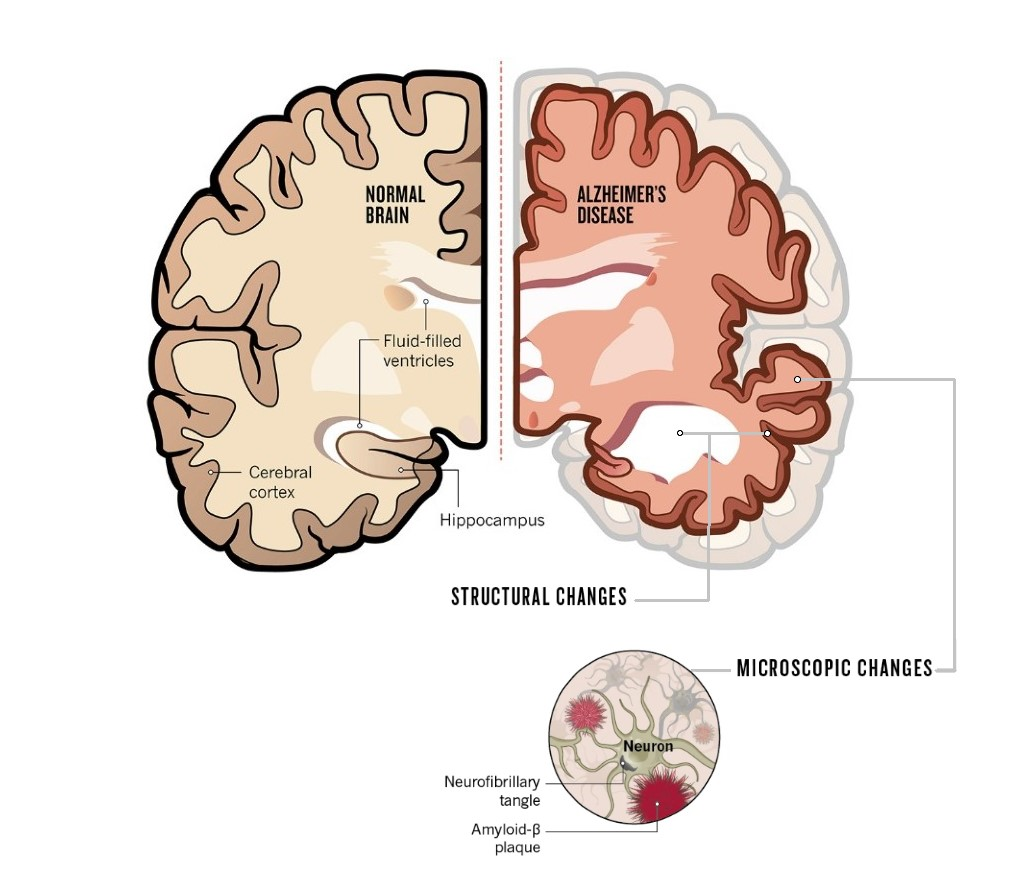
\includegraphics[width=\textwidth]{./imgs/lesiones-cerebrales}
    \caption{Lesiones cerebrales producidas por la enfermedad de Alzheimer.\\Imagen adaptada de una
    ilustración de Stacy Jannis, Alzheimer\'s Association~\cite{nature}.}
    \label{fig:lesiones-cerebrales}
\end{figure}

\section{Fases de la enfermedad}\label{sec:fases-enfermedad}
La EA es una enfermedad de larga evolución en la que, usando una escala de clasificación común, se distinguen
tres fases~\cite{alz-org-etapas}.

\subsection{Enfermedad de Alzheimer leve}\label{subsec:etapa-temprana-EA}
Esta etapa se conoce como etapa temprana y permite al paciente desenvolverse de forma independiente, pero aparecen los
fallos de memoria, como son:
\begin{itemize}
    \item Dificultad para encontrar la palabra o el nombre correctos.
    \item Problemas para realizar tareas en entornos sociales o laborales, destacando la presencia de cambios de
    personalidad.
    \item Olvidarse de algo que acaba de leer.
    \item Problemas para encontrar objetos.
    \item Dificultad para recordar acontecimientos y conversaciones recientes.\\
\end{itemize}

Realizar un diagnóstico de la enfermedad en esta etapa puede ser determinante, ya que existe la posibilidad de aplicar
tratamientos con los que la evolución de la enfermedad pueda ralentizarse sin que resulten perjudiciales para la salud
del paciente.
Sin embargo, es muy difícil realizar el diagnóstico en esta fase pues la mayoría de los síntomas se suelen confundir con
conductas características de la vejez.

\subsection{Enfermedad de Alzheimer moderada}\label{subsec:etapa-media-EA}
En esta etapa media comienzan las limitaciones en las actividades de la vida diaria y la persona con EA necesita un
nivel de atención mayor en tareas básicas como la alimentación o el aseo personal.

La memoria se sigue viendo afectada, de manera más pronunciada en esta etapa, como puede ser dificultad para reconocer a
miembros de la familia, olvidarse eventos o información de la historia personal, o el aumento del riesgo de
desorientarse y perderse en lugares conocidos.

\subsection{Enfermedad de Alzheimer grave}\label{subsec:etapa-final-EA}
En esta etapa final las personas con EA pierden la capacidad de responder a su entorno, sufriendo una pérdida completa
de la memoria y las capacidades intelectuales y funcionales.
Provocando la necesidad de cuidado y asistencia absoluta.
Se produce una pérdida progresiva del lenguaje haciendo que el paciente deje de hablar y una posterior inmovilidad
completa.

La pérdida de las capacidades funcionales hace que se produzca una pérdida de peso y disminución de sus defensas
inmunológicas que conllevan a la muerte.

\section{Diagnóstico de la enfermedad}\label{sec:diagnostico-enfermedad}
Para diagnosticar la EA se requiere de evaluaciones médicas exhaustivas, en las que se evalúa el deterioro de la memoria,
la presencia de cambios de conducta y el estado de otras habilidades de razonamiento, que permitan determinar cuáles son
las capacidades funcionales.
Además, es necesario realizar pruebas médicas que descarten otras posibles causas de deterioro.

El diagnóstico se puede dividir en cuatro partes~\cite{mayo-clinic-diagnostico,alz-org-diagnostico}~:
\begin{itemize}
    \item \textbf{Evaluación del estado mental}: Se evalúan las habilidades de razonamiento (cognitivas) y memoria.
    \item \textbf{Examen físico}: Se evalúa la salud general de la persona, para descartar otras afecciones tratables
    que causen síntomas similares.
    \item \textbf{Examen neurológico}: Se realiza una evaluación de afecciones cerebrales y de salud mental, descartando
    algún trastorno como la depresión.
    \item \textbf{Pruebas de laboratorio} y \textbf{estudios de imágenes cerebrales}.\\
\end{itemize}

\subsection{Pruebas de laboratorio}\label{subsec:pruebas-laboratorio-EA}
Las pruebas de laboratorio incluyen: análisis de sangre para descartar otros trastornos, o examen del líquido
cefalorraquídeo para medir los niveles de proteína amiloide y tau, determinando según su proporción si se trata de EA.
Los exámenes del líquido cefalorraquídeo solo se realizan en casos atípicos y de rápida evolución.

\subsection{Pruebas de diagnóstico por imágenes}\label{subsec:pruebas-imagenes-EA}
Las pruebas de diagnóstico por imágenes ayudan a distinguir diferentes tipos de enfermedades cerebrales degenerativas y
además establecer cuál es el grado de degeneración, por lo que son las pruebas más fiables para el diagnóstico del
Alzheimer.

Las técnicas más frecuentes de diagnóstico por imágenes son:
\begin{itemize}
    \item \textbf{Imagen por Resonancia Magnética (MRI)}: Es una técnica no invasiva que a través de campos magnéticos
    genera imágenes anatómicas tridimensionales.
    Proporciona información exhaustiva de los tejidos blandos y permite examinar la anatomía del cerebro y evaluar
    lesiones presentes.
    \item \textbf{Tomografía Computarizada (más conocida como TAC)}: Con esta técnica se recopilan imágenes transversales
    sucesivas mediante rayos X. Proporciona imágenes óseas, de tejidos blandos y aire y permite identificar anomalías
    asociadas al Alzheimer.
    \item \textbf{Tomografía por emisión de positrones (PET)}: Esta técnica usa radiofármacos de administración intravenosa
    gracias a los cuales se obtienen imágenes de alta definición en las que se pueden detectar y visualizar depósitos
    extracelulares de proteína beta-amiloide.\\
\end{itemize}

\begin{figure}[H]
    \centering
    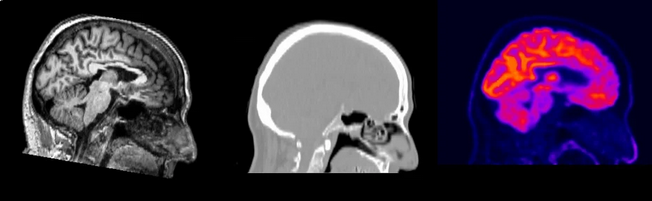
\includegraphics[width=\textwidth]{./imgs/MRI-TAC-PET}
    \caption{Técnicas de diagnóstico por imágenes de la enfermedad de Alzheimer.\\ De izquierda a derecha: MRI, TAC y PET.
    \\Fuente: Fundación Pasqual Maragall~\cite{img-mri-tac-pet}.}
    \label{fig:tecnicas-diagnosico-imagen}
\end{figure}

    \chapter{Estado del arte}\label{ch:estado-del-arte}
En este apartado se incluye la situación actual del uso de técnicas de DL para el diagnóstico del Alzheimer, es decir,
la información sobre las últimas actualizaciones e investigaciones ya disponibles al público sobre este tema.

En la última década, las técnicas de aprendizaje profundo han alcanzado una enorme popularidad en el ámbito del análisis
de imágenes médicas y como herramienta de diagnóstico y seguimiento de enfermedades.
Al mismo tiempo, ha incrementado el uso de técnicas de neuroimagen para el diagnóstico de la EA, por lo que la unión de
ambas técnicas, de aprendizaje profundo y de neuroimagen, ha demostrado ser una combinación ideal para realizar un
correcto diagnóstico de la enfermedad y poder predecir la evolución de la misma.

El número de artículos de investigación de la detección de la EA que se han publicado en los últimos años ha crecido
exponencialmente.
Recogiendo información sobre múltiples resultados con el uso de distintos biomarcadores o distintos modelos profundos.

La mayoría de los artículos publicados tratan el tema de la misma manera: planteando un nuevo modelo de aprendizaje
profundo y no llegando a explorar mejoras a otras alternativas o reflexionar sobre qué recursos son mejores, siendo el
resultado un cúmulo de estudios que no producen una conclusión concreta a qué métodos son más óptimos y por qué.
Existe un artículo de la universidad en Newcastle, Australia, que realiza una revisión de la literatura de más de 100
artículos y que detalla los hallazgos y tendencias, examinando biomarcadores y características útiles, técnicas de
preprocesamiento necesarias y diferentes métodos de tratamiento de neuroimágenes~\cite{literature-review}.
Este estudio se ha utilizado de referencia para este apartado.

\section{Biomarcadores que intervienen en la detección de la EA}\label{sec:biomarcadores-estado-del-arte}
Para la detección de la EA las técnicas de neuroimagen no invasivas más utilizadas en los estudios son: MRI, fMRI
(Imagen por resonancia magnética funcional)  y PET.

La fMRI es un tipo especial de MRI que proporciona un conjunto de imágenes del flujo sanguíneo de ciertas partes del
cerebro y también son utilizadas para evaluar daños cerebrales~\cite{mayo-clinic-mri}.

De estas técnicas, MRI es el biomarcador más utilizado en la literatura debido a que ha demostrado un alto rendimiento.
A pesar de que varios estudios han demostrado que la MRI es más discriminatoria en comparación con la PET, otros estiman
que la MRI es igual de discriminatoria que la PET o ligeramente menos.

Además MRI es la técnica más frecuente en las pruebas médicas para la detección de la EA ya que proporciona información
precisa y el coste de su realización es menor.
Lo que sitúa a esta técnica como la mejor candidata para avanzar en la investigación del diagnóstico de la enfermedad.

\section{Técnicas de preprocesamiento de biomarcadores}\label{sec:preprocesamiento-estado-del-arte}
La mayoría de los trabajos de investigación, en especial los de ML, necesitan aplicar un preprocesamiento a los datos
antes de poder manejarlos.
Con el uso de técnicas de DL, algunos pasos de preprocesamiento no son tan cruciales, no obstante, en la mayoría de
casos, se realiza un preprocesamiento de los datos.
Las técnicas de preprocesamiento más usadas son:
\begin{itemize}
    \item Normalización de la intensidad.
    \item Registro de la imagen.
    \item Segmentación del tejido.
    \item Segmentación del cráneo.
    \item Corrección del movimiento.\\
\end{itemize}

\section{Técnicas de análisis de neuroimagen}\label{sec:analisis-de neuroimagen-estado-del-arte}
Las técnicas de análisis o de extracción de características en neuroimagen se pueden dividir en cuatro categorías,
dependiendo de las características extraídas: basadas en vóxeles, en cortes, en parches y en regiones de interés
(en adelante \Gls{ROI}).

\textbf{La técnica basada en vóxeles}, también llamada morfometría basada en Vóxel (VBM), es la más sencilla, se utiliza en MRI,
permite el análisis de lesiones focales cerebrales y en ella se realiza una división del cerebro en vóxeles que son la
unidad cúbica que compone un objeto tridimensional, el equivalente al píxel en un objeto bidimensional.
Esta técnica permite identificar las diferencias de concentración entre la sustancia gris y la sustancia blanca del
cerebro mediante la comparación vóxel a vóxel de los valores de intensidad de los mismos.

\textbf{La técnica basada en cortes} consiste en extraer, mediante cortes, imágenes bidimensionales con la mayor información
posible.
Ya que el uso de las tres vistas de las neuroimágenes tridimensionales puede proporcionar características
útiles adicionales para la clasificación, algunos estudios tienen en cuenta todas las vistas de la imagen (sagital,
coronal y axial).

En \textbf{la técnica basada en parches}, pequeños sub-volúmenes de la imagen definidos como cubos tridimensionales conocidos
como parches se usan para extraer patrones relacionados con la enfermedad.
La diferencia entre un parche y un vóxel es que los vóxeles constituyen la mínima unidad procesable.

La \textbf{técnica basada en ROI} se centra en las partes del cerebro más afectadas en la fase temprana de la EA, en vez de
ocuparse de todo el cerebro.

Las conclusiones obtenidas en la literatura sobre las técnicas de análisis en neuroimagen son las siguientes:
\begin{itemize}
    \item Los métodos basados en ROI y en parches son más exactos, ya que son los métodos con los que se obtiene
    información más relevante;
    sin embargo, son también los métodos más costosos.
    \item Los métodos basados en parches son más precisos que los basados en vóxeles, pero la selección de los parches
    con más información de la imagen es una tarea compleja.
    \item El uso de cortes 2D como entrada en lugar de la imagen 3D en su totalidad evita la generación de millones de
    parámetros de entrenamiento e induce a la simplificación de las redes a costa de perder información.
    \item Al utilizar métodos basados en cortes, las vistas sagital y coronal resultan ser las más discriminatorias,
    aunque las vistas axiales son las más utilizadas.
    Hay estudios que afirman que no hay diferencias significativas entre planos.\\
\end{itemize}

\section{Modelos profundos más utilizados para obtener patrones relacionados con la EA}
\label{sec:modelos-profundos-estado-del-arte}
Lamentablemente la mayoría de los estudios no publican su código fuente por lo que resulta difícil comparar de manera
imparcial los estudios entre sí.
Además, normalmente los artículos se limitan a comparar precisiones finales y no a comparar distintos factores como el
coste computacional.

Las redes neuronales convolucionales (en adelante \Gls{CNN}) son las más usadas en el ámbito de la medicina porque han
demostrado una alta precisión en términos de clasificación de imágenes médicas.

Entre los modelos observados, los mejores resultados se encuentran entre las 3D-CNN y las 2D-CNN. Ambas opciones tienen
un buen rendimiento para la extracción de características, en el caso de las arquitecturas de red neuronal de tipo
3D-CNN estas muestran ligeramente un mayor rendimiento, ya que recogen información tridimensional y, por tanto, más
cantidad de información;
sin embargo, las de tipo 2D-CNN son más fáciles de entrenar, requieren de un menor coste computacional.

En cuanto a arquitecturas 2D-CNN: Inception-V4, ResNet y CaffeNet han superado a GoogLeNet, VGGNet-16 y AlexNet.

En la mayor parte de los estudios se entrena un modelo profundo desde cero, pero, esto puede ser ineficiente, porque
el proceso de entrenamiento requiere mucho tiempo y un gran conjunto de datos.
Mientras que los conjuntos de datos para la detección y clasificación de objetos genéricos cuentan con millones de
imágenes, los conjuntos de datos de neuroimagen disponibles del seguimiento de la EA suelen ser pequeños, de solo
cientos de imágenes, lo que da lugar a un sobreajuste.
El Transfer Learning (en adelante \Gls{TL}) es más rápido y alcanza mejores resultados que el entrenamiento desde cero, de
modo que, generalmente resulta útil utilizar CNNs probadas y pre-entrenadas para volver a entrenarlas con otro conjunto
de datos.

\section{Conjuntos de datos y herramientas de software útiles}\label{sec:datos-y-herramientas-estado-del-arte}
Como paquetes software de análisis de neuroimagen están:
FreeSurfer\footnote{~\cite{freeSurfer}{FreeSurfer}},
FSL\footnote{~\cite{fsl}{Functional magnetic resonance imaging of the brain Software Library (FSL)}},
MIPAV\footnote{~\cite{mipav}{Medical Image Processing, Analysis, and Visualization (MIPAV)}}
y SPM\footnote{~\cite{spm}{Statistical Parameter Mapping (SPM)}},
que ofrecen herramientas potentes para diversas técnicas de preprocesamiento automatizado comentadas en el
apartado~\ref{sec:preprocesamiento-estado-del-arte}.

Para implementar modelos profundos las herramientas más utilizadas son:
MATLAB\footnote{~\cite{matlab}{MATLAB}}
Keras\footnote{~\cite{keras}{Keras}},
TensorFlow\footnote{~\cite{tensorflow}{TensorFlow}},
Theano,
Caffe\footnote{~\cite{caffe}{Caffe}},
y Torch\footnote{~\cite{torch}{Torch}}.
Siendo Keras y TensorFlow los más utilizados y Torch el menos utilizado.

La principal dificultad a la que se enfrentan los investigadores es la falta de imágenes que permitan formar un gran
conjunto de datos de entrenamiento con el que poder obtener un resultado preciso y, por tanto, un diagnóstico fiable.
La escasez de datos es un problema que se debe a las restricciones de privacidad de las imágenes médicas y de su elevado
coste en muchos casos.

Como bases de datos online para obtener conjuntos de datos relativos a la EA, las más importantes son:
ADNI\footnote{~\cite{adni}{Alzheimer’s Disease Neuroimaging Initiative (ADNI)}},
AIBL\footnote{~\cite{aibl}{Australian Imaging, Biomarker and Lifestyle (AIBL)}},
OASIS\footnote{~\cite{oasis}{Open Access Series of Imaging Studies (OASIS)}}
y MIRIAD\footnote{~\cite{miriad}{Minimal Interval Resonance Imaging in Alzheimer's Disease (MIRIAD)}},
que ofrecen al público biomarcadores como neuroimagen, información genética y sanguínea, y evaluaciones
clínicas y cognitivas.
ADNI es la que más destaca de todas ellas por ser un estudio multicéntrico y longitudinal, además es el más común en la
literatura, de manera individual o en combinación con otros.
Esta última es una forma de poner solución a la insuficiencia de datos.
Al combinar diferentes conjuntos de datos, se produce una mayor heterogeneidad, lo cual es una desventaja, pero se crea
un modelo amplio para la clasificación y la predicción.

Las técnicas de aumento de datos entre las que se encuentran la reflexión, la rotación, la traslación aleatoria, el
desenfoque o el escalado mejoran el rendimiento de la clasificación sin la necesidad de recoger nuevos datos cuando
estos son limitados.

Se recomienda el uso de un conjunto de datos equilibrado, ya que, en caso contrario, un desequilibrio entre pacientes de
distintas categorías provoca una variación en la precisión.
Siendo, por tanto, preferible el uso de un conjunto de datos menor antes que uno desequilibrado.

    \chapter{Análisis y Desarrollo Experimental}\label{ch:analisis-y-desarrollo-experimental}
En este capítulo se recoge el estudio de técnicas del DL para el diagnóstico del Alzheimer, pasando por las 
herramientas y los datos utilizados hasta la experimentación y el análisis de los resultados obtenidos.

\section{Presentación del problema a resolver}\label{sec:presentacion-del-problema-a-resolver}
Tras la investigación del estado actual de la literatura en este ámbito, se recopilan los siguientes puntos sobre el DL
para clasificación de la EA:

\begin{itemize}
    \item El Transfer Learning es la mejor técnica de entrenamiento.
    \item Los datasets balanceados ofrecen mejores resultados, y más fiables, en la clasificación de imágenes,
    pero la limitación de disponibilidad de biomarcadores del seguimiento de la EA puede suponer un obstáculo.
    \item La prueba más frecuente para el diagnóstico de la enfermedad es la MRI.
    \item No se clarifica qué plano cerebral (axial, coronal o sagital) es mejor utilizar y bajo qué diferencias de
    rendimiento.
    \item No se realizan comparativas de rendimiento entre distinto número de clases. \\
\end{itemize}

Se propone desarrollar un sistema de aprendizaje profundo a partir de MRI con el cual:

\begin{itemize}
    \item Realizar un análisis sobre qué plano cerebral ofrece mejores resultados en el diagnóstico de la EA, ya que se
    tiene en cuenta que las redes neuronales de 3 dimensiones requieren de una capacidad computacional muy alta.
    \item Realizar una comparativa del rendimiento de la clasificación entre 2 y 3 clases: Cognitivamente normal frente 
    a Alzheimer y cognitivamente normal frente a deterioro cognitivo leve frente Alzheimer. \\
\end{itemize}

\section{Conjunto de datos empleado}\label{sec:conjunto-de-datos-empleado}
El conjunto de biomarcadores MRI que se ha utilizado se ha obtenido de la base de datos ADNI, que es un estudio
longitudinal multicéntrico en el que se desarrollan biomarcadores genéticos, bioquímicos y de imagen para la detección
temprana y el seguimiento de la EA, se habla más en profundidad sobre esta base de datos en el
apartado~\ref{ch:aped.a}.
Cabe destacar que también intentó hacer uso de la base de datos OASIS, de forma que se obtuviera un número mayor de
datos y poder prevenir los posibles problemas por falta de datos, pero no fue posible ya que no se aprobó la solicitud
de acceso realizada.

Para la selección de los biomarcadores MRI a utilizar se han dividido 3 grupos de investigación según el grado de EA
del sujeto, diferenciándose:
\begin{itemize}
    \item \textbf{Cognitivamente normal} (en adelante este grupo se denominará \textbf{CN}): Sujetos sanos.
    \item Sujetos con un \textbf{deterioro cognitivo leve}, del inglés Mild Cognitive Impairment (en adelante este grupo
    se denominará \textbf{MCI})
    \item Sujetos con \textbf{Alzheimer} diagnosticado (en adelante este grupo se denominará \textbf{AD}). \\
\end{itemize}

Para la realización de la experimentación se han utilizado biomarcadores MRI de tipo \textit{NIfTI} pertenecientes a un
subconjunto de datos sometidos a un post-procesamiento que se comenta en la sección~\ref{subsec:post-procesamiento-en-adni}.

En el subconjunto de datos disponibles, los biomarcadores de clase \Gls{AD} son más limitados que los de clase \Gls{CN} y \Gls{MCI}.
Siendo la distribución de los datos la siguiente:

\begin{figure}[H]
    \centering
    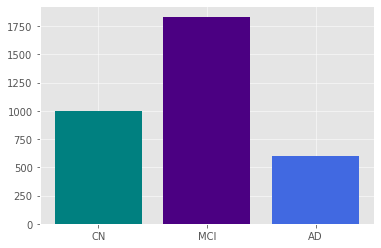
\includegraphics[width=0.6\textwidth]{./imgs/histograma-de-clases}
    \caption{Histograma de clases}
    \label{fig:histograma-de-clases}
\end{figure}

Como se puede apreciar en la Figura~\ref{fig:histograma-de-clases}, existe un desbalance de clases, habiendo 998
neuroimágenes de tipo CN, 1832 de tipo MCI y 602 de tipo AD.

Para realizar el entrenamiento con un datasets balanceado se utilizan todos los datos de tipo AD disponibles y se
realiza un submuestreo de las clases mayoritarias para equilibrar las clases.
El uso de la técnica de submuestreo presenta una desventaja ya que se pierde información, pero se elige esta técnica
frente a la técnica de sobremuestreo, ya que esta última consiste en aumentar los datos de la clase minoritaria, lo
que puede llevar a un sobreajuste y teniendo en cuenta que ya el conjunto de datos general del que se dispone es muy
limitado y es posible que se obtenga un sobreajuste no se quieren multiplicar las posibilidades.

De modo que el conjunto completo de datos balanceado que se utiliza para extraer los cortes axial, coronal y sagital
está formado por \textbf{1806} neuroimágenes en total.

\section{Herramientas utilizadas}\label{sec:herramientas-utilizadas}
Para realizar este estudio es necesario utilizar una serie de herramientas que faciliten y hagan posible la 
experimentación.
Hay que tener en cuenta dos grupos de herramientas: Las herramientas para trabajar con biomarcadores de tipo MRI y las 
herramientas para trabajar con técnicas de DL.

\subsection{Herramientas para trabajar con biomarcadores MRI de tipo NIfTI}
\label{subsec:herramientas-para-trabajar-con-biomarcadores-mri-de-tipo-nifti}
Para poder realizar el sistema de clasificación es necesario realizar un procesamiento de los archivos de MRI, de 
manera que se obtengan cortes de 2 dimensiones a partir del archivo en 3 dimensiones.
Para conseguirlo se ha hecho uso de la librería para python \textbf{NiBabel}, que permite la lectura y escritura  de 
archivos de neuroimagen, en nuestro caso del formato \textit{NIfTI}.
Por lo que mediante esta librería se puede cargar una MRI, extraer el corte o slice deseado y guardarlo.

Además, para la visualización de este tipo de archivos se requiere de software de visualización de imágenes específico.
Hay múltiples herramientas disponibles para ello según la finalidad que se quiera conseguir.
Para visualizar archivos en formato \textit{NIfTI} se ha hecho uso del software \textbf{MRIcron}, que ha requerido 
instalación y con el que se ha podido realizar una visualización de múltiples capas de la MRI. También se ha hecho uso 
del recurso \textbf{IDA} online del que se obtienen los datos de la base de datos \textit{ADNI} y del que se detalla más
información en el el apartado~\ref{ch:aped.a}.
Este recurso integra un visualizador de neuroimágenes.


\subsection{Herramientas para trabajar con técnicas de Deep Learning}
\label{subsec:herramientas-para-trabajar-con-tecnicas-de-deep-learning}
Como bien se muestra en el apartado~\ref{sec:datos-y-herramientas-estado-del-arte}, existe un amplio abanico de
posibilidades en cuanto a herramientas que permiten la experimentación de técnicas de DL.

De entre todas ellas se ha optado por utilizar \textbf{TensorFlow} y \textbf{Keras}, no solo por ser las más utilizadas
en la literatura, sino también porque son las que ofrecen una mejor documentación para su uso.

Para trabajar con imágenes 2D y por lo tanto con vectores y matrices se hace uso de la biblioteca de \textit{Python}
\textbf{NumPy}.

Para visualizar, tanto las imágenes de los planos cerebrales obtenidos como para la representación de las gráficas de
resultados se usa \textbf{Matplotlib}.

Para obtener las métricas para evaluar los resultados obtenidos del entrenamiento se hace uso de la librería
\textbf{scikit-learn}.

Por lo tanto el lenguaje de programación con el que se va a trabajar en este TFG y en concreto en el desarrollo
experimental es \textbf{Python}.

\section{Procesamiento de biomarcadores}\label{sec:procesamiento-de-biomarcadores}

\subsection{Post-procesamiento en ADNI}\label{subsec:post-procesamiento-en-adni}
Tal y como se ha comentado en ~\ref{sec:conjunto-de-datos-empleado}, el conjunto de datos utilizado en este estudio se
ha obtenido de un subconjunto de neuroimágenes de ADNI al que se le aplica un procesamiento, con el objetivo de extraer
la información más importante y descartar la irrelevante.

Para la realización de este procesamiento, al que ADNI denomina como post-procesamiento, ya que se  en una fase
posterior a la examinación del sujeto, se hace uso de la herramienta FreeSurfer y  se aplican las siguiente técnicas:

\begin{itemize}
    \item \textbf{Registro de la imagen}: proceso de transformación a un sistema de coordenadas común.
    Consiguiendo que en distintas imágenes cerebrales los í correspondan en posición.
    \item \textbf{Segmentación del cráneo}: proceso de eliminación del cráneo para aislar la masa cerebral.
    \item \textbf{Normalización de la intensidad}: proceso de corrección de intensidad de la imagen.
    Se aplica N3 que es un algoritmo de afilado de picos de histograma. \\
\end{itemize}

En la Figura~\ref{fig:adni-mri} se puede ver una comparativa entre una MRI en bruto con MP-RAGE y la misma post-procesada con
FreeSurfer.

\begin{figure}[H]
    \centering
    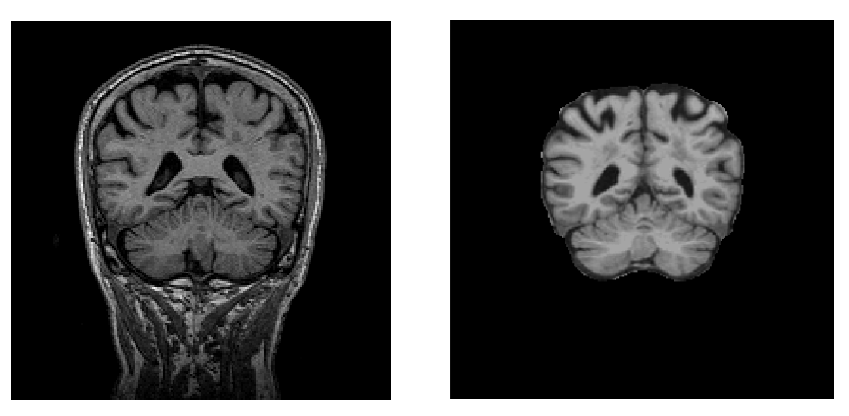
\includegraphics[width=\textwidth]{./imgs/adni-mri}
    \caption{Técnicas de procesamiento de MRI en ADNI. De izquierda a derecha: MRI en bruto con MP-RAGE y MRI
    post-procesada con FreeSurfer. Fuente: Alzheimer’s Disease Neuroimaging Initiative~\cite{img-adni-mri}. }
    \label{fig:adni-mri}
\end{figure}

\subsection{Creación de las imágenes para el entrenamiento}\label{subsec:creacion-de-las-imagenes-para-el-entrenamiento}
Para evaluar qué plano cerebral ofrece mejores resultados para el diagnóstico de la EA a partir de biomarcadores MRI es
necesario obtener imágenes 2D a partir de los archivos de MRI \textit{NIfTI}.

\begin{figure}[H]
    \centering
    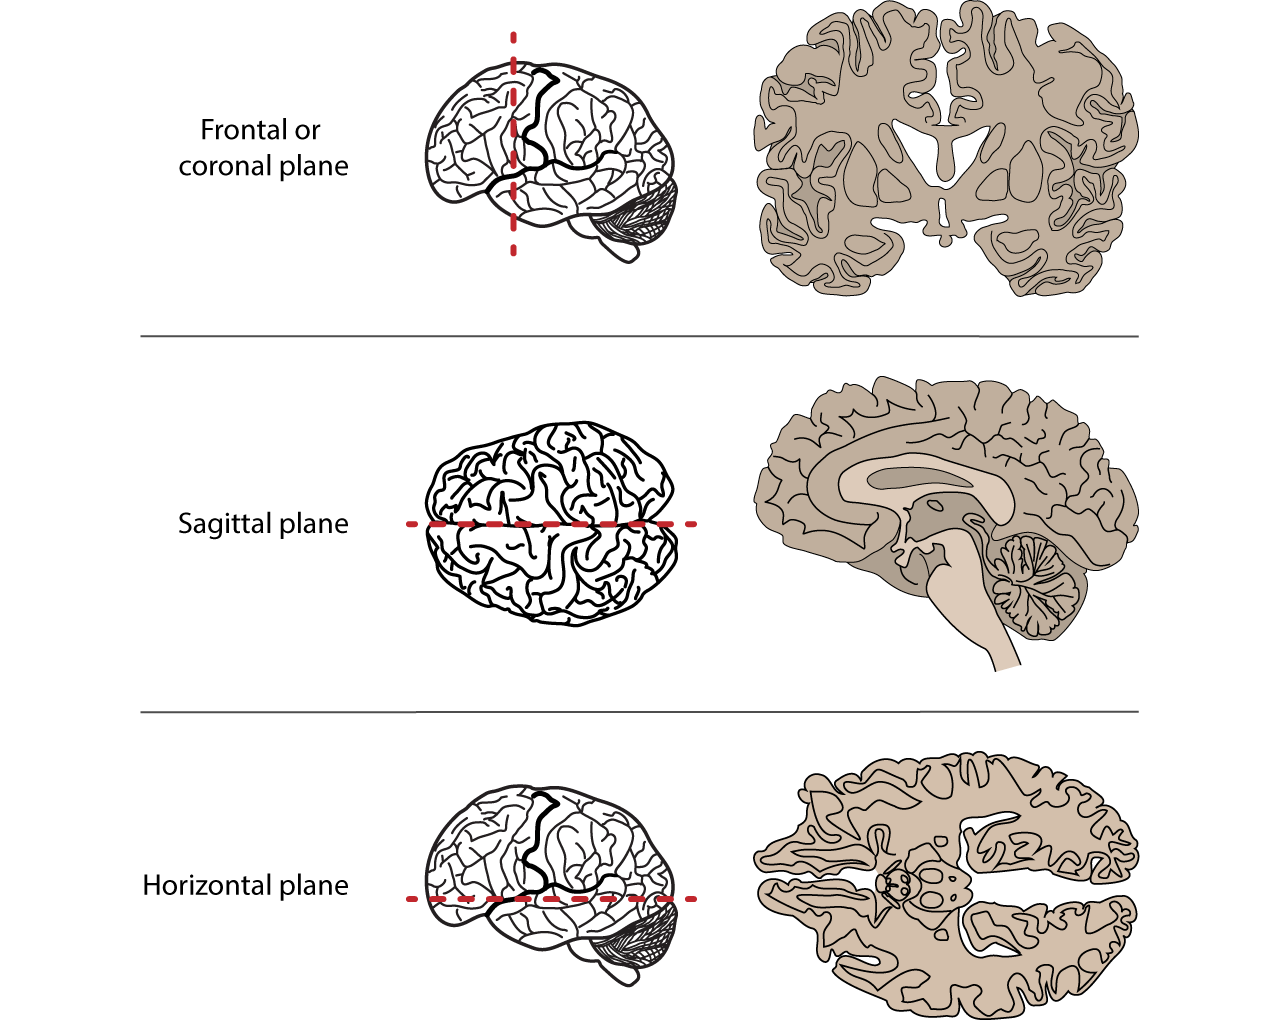
\includegraphics[width=\textwidth]{./imgs/planos-cerebrales}
    \caption{Planos Cerebrales. Fuente: Anatomical Planes por Casey Henley~\cite{img-planos-cerebrales}. }
    \label{fig:planos-cerebrales}
\end{figure}

Para ello mediante un script de python se leen las imágenes 3D, se generan los cortes correspondientes a los planos
usando la capa de central como corte del plano para extraer la mayor información posible y se guardan los cortes
generados en carpetas dedicadas a cada plano.

De manera que el conjunto de resonancias magnéticas del que se extraen los cortes es el mismo para los tres subconjuntos
que se obtienen.
De esta forma se garantiza que a la hora de concluir la evaluación, los cortes han surgido de las mismas resonancias
magnéticas y los resultados serán fiables.

\begin{figure}[H]
    \centering
    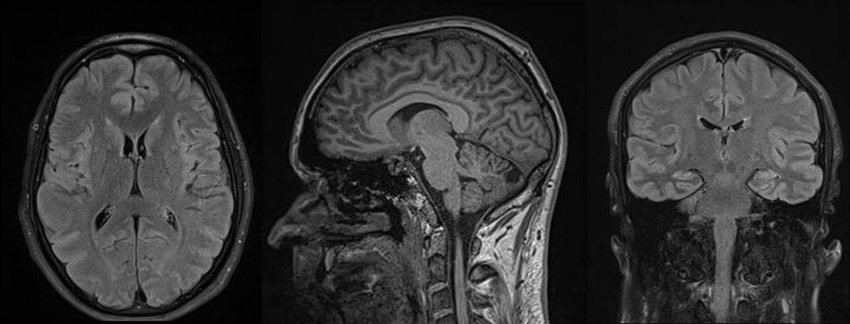
\includegraphics[width=\textwidth]{./imgs/MRI-planos-cerebrales}
    \caption{MRI en los planos axial, sagital y coronal.
    Fuente: Trakia Journal of Sciences~\cite{img-mri-planos-cerebrales}. }
    \label{fig:mri-planos-cerebrales}
\end{figure}

\section{Estrategias de entrenamiento}\label{sec:estrategias-de-entrenamiento}
Tras la conclusión de la revisión de la literatura se ha decidido aplicar en este estudio las técnicas de Transferencia
de Aprendizaje o Transfer Learning (en adelante TL) y Aumento de datos o Data Augmentation.
En este apartado se explica el fundamento de ambas técnicas.

\subsection{Transfer Learning}\label{subsec:transfer-learning}
El TL es una técnica que consiste en utilizar modelos probados y pre-entrenados, con un conjunto de datos igual o
distinto al problema a resolver, para volver a entrenarlos con el conjunto de datos relativos al problema.
De modo que se requiere menos tiempo de cálculo o recursos que si se construye el modelo desde cero.

Tal y como se ha concluido en la revisión de la literatura, esta técnica es útil y ofrece un gran número de ventajas,
por lo tanto en este estudio se ha aplicado esta técnica utilizando una arquitectura pre-entrenada con los pesos de
\textit{ImageNet}.

En cuánto a la forma de aplicar TL se ha optado por aplicar \textit{fine-tuning} ya que al utilizar esta técnica se
aprovechan las ventajas que aporta el uso de transferencia de aprendizaje para conjuntos de datos distintos a los del
entrenamiento original.
Para ello los pasos son:
\begin{itemize}
    \item Se crea el modelo base pre-entrenado.
    \item Se reconstruye la parte superior del modelo adaptándola al problema que se quiera solucionar.
    \item Se congela la base convolucional para la extracción de características.
    \item Se entrena el modelo sólo con los pesos de la última capa, de manera que se aprovechan las características
    aprendidas en la última capa para la resolución del problema.
    \item Se descongelan las capas superiores del modelo, se escoge la capa desde la que quiere aplicar
    \textit{fine-tuning} y se congelan todas las capas previas a esa.
    \item Se re-entrena el modelo durante un número de épocas con el objetivo de aumentar la precisión del modelo.\\
\end{itemize}

\subsection{Data Augmentation}\label{subsec:data-augmentation}
Esta técnica consiste en aumentar la diversidad del conjunto de entrenamiento mediante la aplicación de transformaciones
aleatorias pero realistas.

Las técnicas de aumento de datos han demostrado una mejora del rendimiento de la clasificación sin la necesidad de
recoger nuevos datos cuando estos son limitados, y teniendo en cuenta que para este estudio los datos disponibles son
reducidos, se opta por aplicarla en la experimentación.

\section{Arquitectura del modelo profundo utilizado}\label{sec:arquitectura-del-modelo-profundo-utilizado}
Se ha elegido \textbf{EfficientNetB7} como modelo pre-entrenado porque es el modelo de aprendizaje profundo pre-entrenado
con mejor rendimiento que ofrece Keras~\cite{keras-applications}.

Las \textit{EfficientNets} son una familia de modelos de clasificación de imágenes que alcanzan una alta precisión,
pero siendo en orden de magnitud más pequeños y rápidos que otros modelos~\cite{efficientnets}.

\begin{figure}[H]
    \centering
    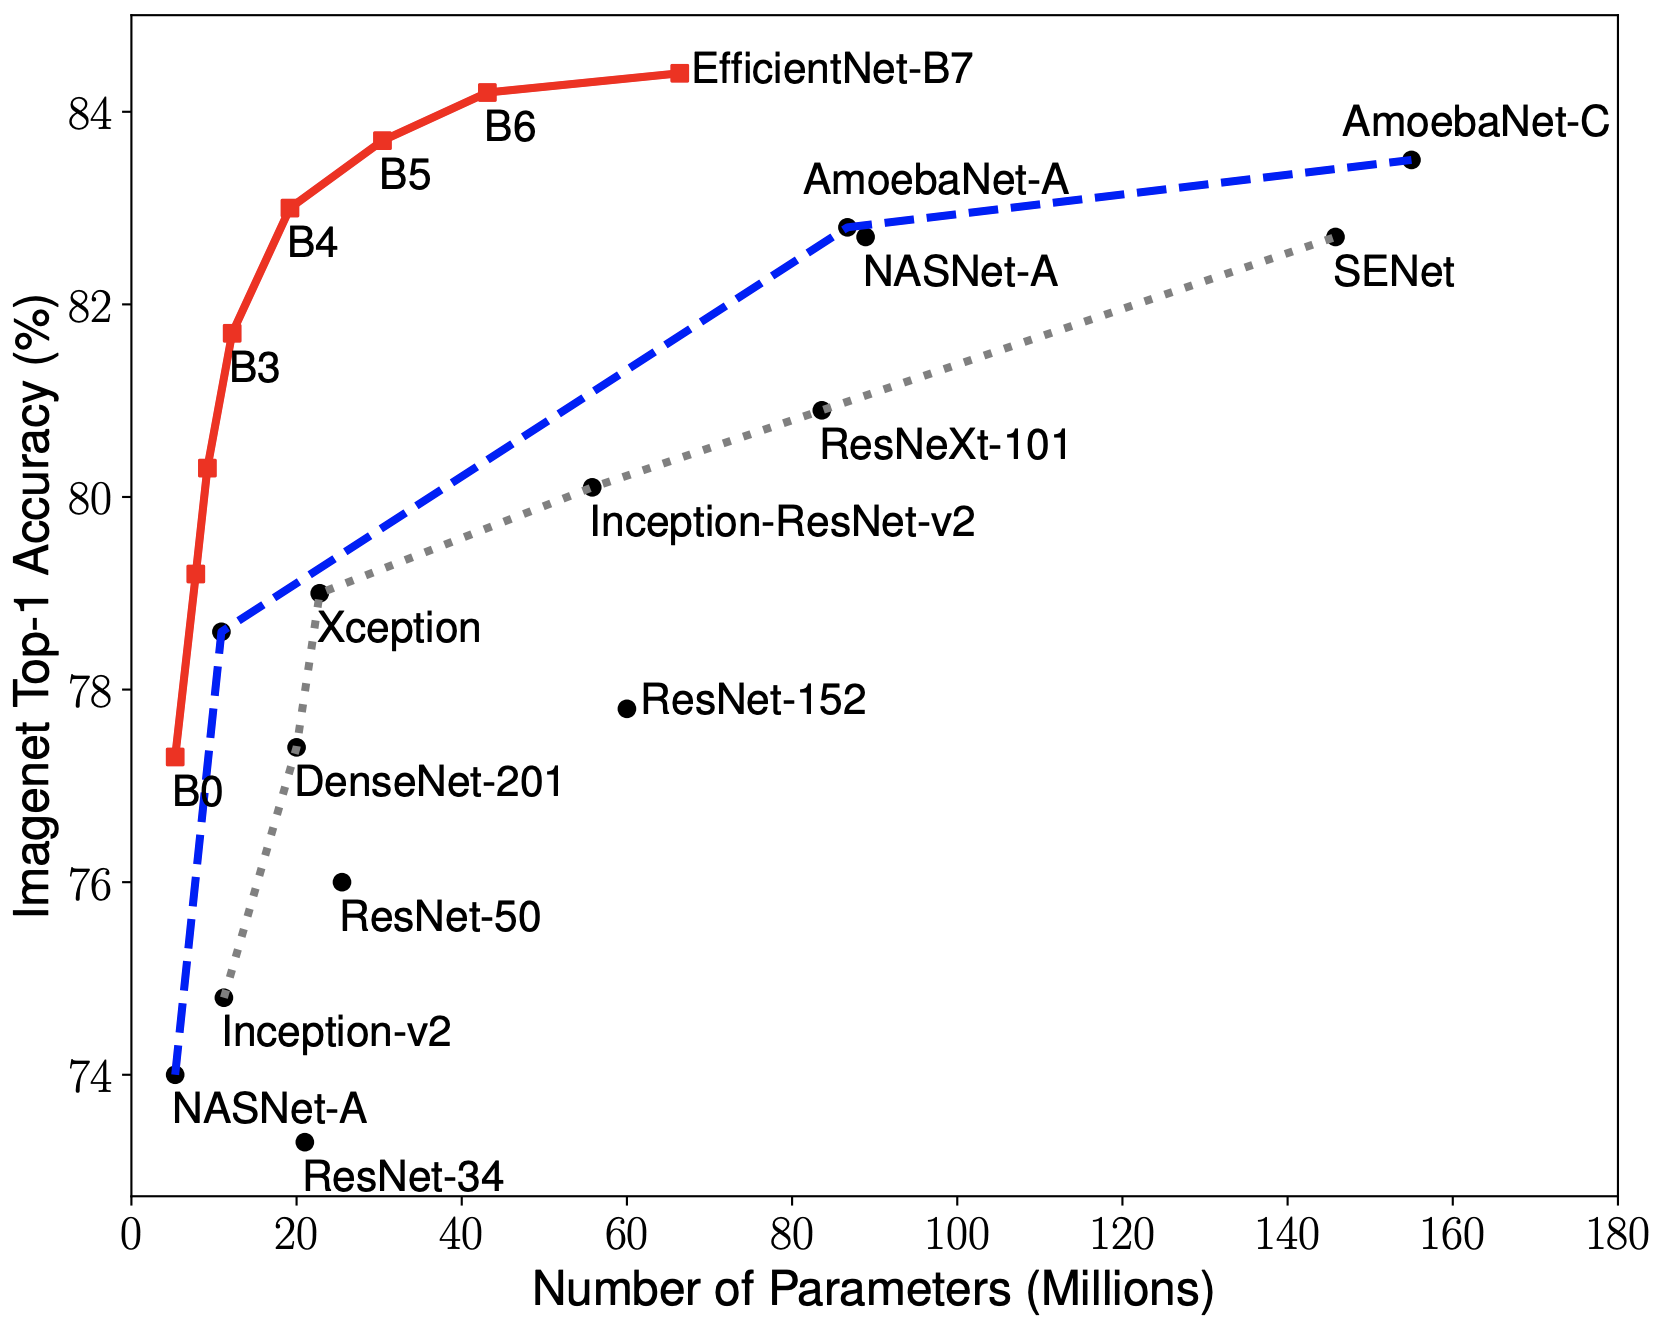
\includegraphics[width=0.5\textwidth]{./imgs/redimiento-efficientnet}
    \caption{Rendimiento de EfficientNet en comparación con otras arquitecturas. Fuente:~\cite{efficientnets-models}. }
    \label{fig:redimiento-efficientnet}
\end{figure}

\begin{figure}[H]
    \centering
    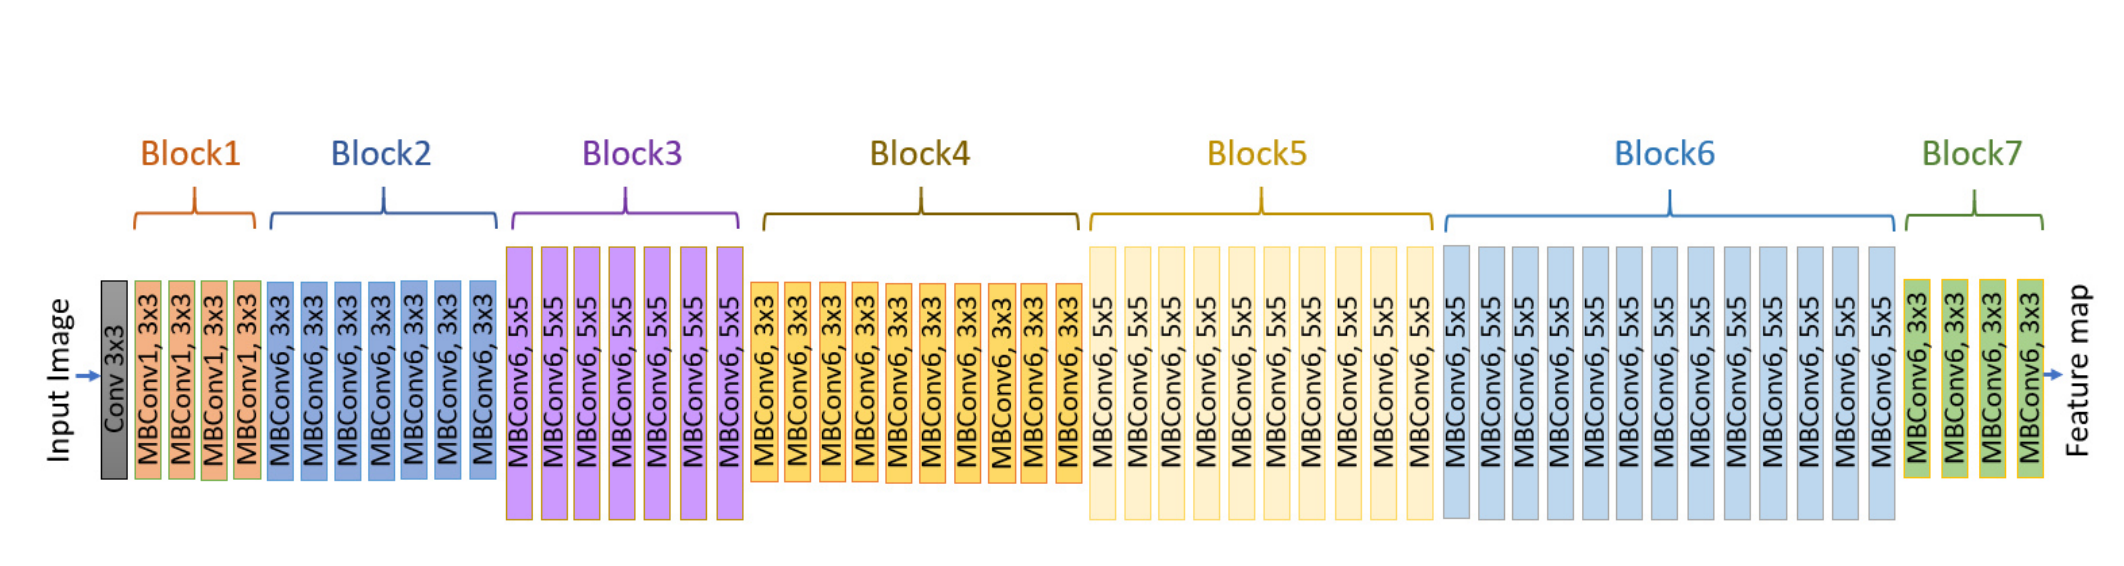
\includegraphics[width=\textwidth]{./imgs/efficientnetb7-model-architecture}
    \caption{Arquitectura del modelo EfficientNetB7. Fuente:~\cite{efficientnetb7-model-architecture}. }
    \label{fig:efficientnetb7-model-architecture}
\end{figure}

\section{Estrategia de entrenamiento}\label{sec:estrategia-de-entrenamiento}
En este caso al aplicar \textit{fine-tuning}, a la hora de reconstruir la parte superior del modelo, se han añadido las
siguientes capas con el objetivo de prevenir y reducir el \textit{overfitting} o \textit{sobreajuste}:
\begin{itemize}
    \item Capa Global Average Pooling para la regularización estructural y evitar el sobreajuste de la estructura global.
    \item Capa Dropout con un  rate de 0.3 para que nuestro modelo sea más robusto.
    \item Capa Batch Normalization para mejorar el funcionamiento, velocidad y estabilidad. \\
\end{itemize}

En cuanto a la aplicación de Data Augmentation, se ha incluido como capa de preprocesamiento del modelo formando parte
del mismo, de esta forma a la hora de exportar el modelo e implementarlo, se estandarizarán de manera automática las
imágenes evitando que haya que repetir este preprocesamiento en el lado del servidor.
Lo que resulta una ventaja de cara a la implementación de la aplicación web que forma parte de este proyecto.

Para aumentar el conjunto de entrenamiento se ha incluido una capa para rotar la imagen y otra para voltear horizontal
y verticalmente.

También se incluye en la capa de preprocesamiento del modelo un redimensionado de las imágenes a 224×224 píxeles para
no causar conflictos con la entrada del modelo base.

Al aplicar TL se han seguido los pasos comentados en el apartado~\ref{subsec:transfer-learning} y se ha utilizado de
referencia el análisis de la literatura y la documentación de Keras y TensorFlow.
De modo que se ha definido un tamaño de \textit{batch} de 32, se han establecido el número de épocas iniciales y de re-entreno
a 10, formando un total de épocas de 20 y la capa en la que se va a aplicar \textit{fine-tuning} a 20.
El valor de la tasa de aprendizaje utilizado en la primera fase se ha establecido con un rate de 0.0001 y en la segunda
fase 0.00001, haciendo uso del optimizador Adam (Adaptive moment estimation) en la primera fase y
RMSprop (Root Mean Square Propagation) en la segunda.


\section{Experimentos}\label{sec:experimentos}
En esta sección se muestran los resultados obtenidos.
Se ha utilizado el mismo modelo para hacer la comparativa, cambiando únicamente los datos de entrenamiento en base a
cada caso.

\subsection{Análisis de resultados}\label{subsec:analisis-de-resultados}
Para realizar la evaluación de los resultados y obtener una conclusión al estudio se va a utilizar de
métrica la precisión o \textit{accuracy}.

    \[accuracy=\frac{VP+VN}{VP+VN+FP+FN}\]

La precisión establece qué porcentaje de datos han sido etiquetados de forma correcta por el modelo.
Siendo \textit{VP} y \textit{VN} los verdaderos positivos y verdaderos negativos respectivamente,
y \textit{FP} y \textit{FN} los falsos positivos y falsos negativos respectivamente.

Puesto que el dataset con el que se trabaja en este estudio está balanceado esta métrica es relevante para realizar
la evaluación.

Además de cada caso se va a incluir la evolución del modelo durante el entrenamiento, la matriz de confusión y el
Informe de clasificación o o \textit{Classification Report}.


\subsection{Resultados del plano Axial}\label{subsec:resultados-del-plano-axial}

\begin{figure}[H]
    \centering
    \begin{subfigure}{0.45\textwidth}
        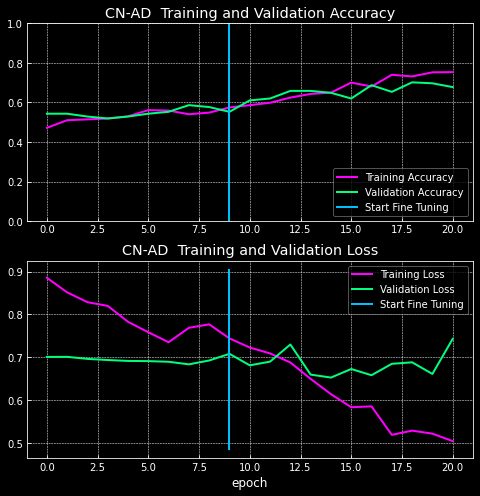
\includegraphics[width=\textwidth]{./imgs/resultados/axial/CN_AD_output_AXIAL}
        \caption{Comparativa CN-AD. }
        \label{fig:axial-cn-ad}
    \end{subfigure}
    \hspace*{\fill}
    \begin{subfigure}{0.45\textwidth}
        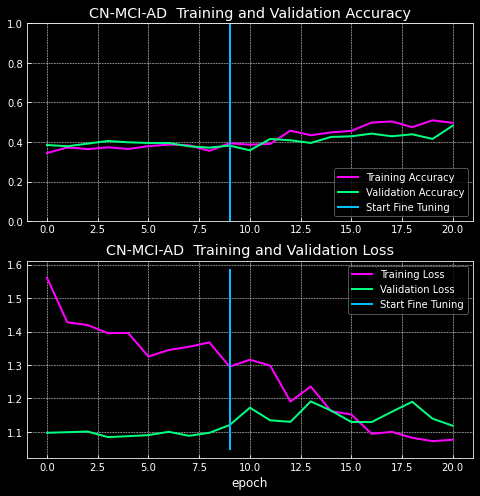
\includegraphics[width=\textwidth]{./imgs/resultados/axial/CN_MCI_AD_output_AXIAL}
        \caption{Comparativa CN-MCI-AD. }
        \label{fig:axial-c-mci-ad}
    \end{subfigure}
    \caption{Evolución del modelo durante el entrenamiento: plano Axial} \label{fig:axial-model}
\end{figure}

\begin{table}[H]
    \centering
    \begin{tabular}{r r r r r}
        & precision & recall & f1-score & support \\
        AD & 0.70 & 0.50 & 0.58 & 14 \\
        CN & 0.68 & 0.83 & 0.75 & 18 \\
        & & & & \\
        accuracy &  &  & 0.69 & 32 \\
        macro avg & 0.69 & 0.67 & 0.67 & 32 \\
        weighted avg & 0.69 & 0.69 & 0.68 & 32 \\
    \end{tabular}
    \caption{Classification Report del plano Axial. Comparativa CN-AD}
    \label{tab:cr-axial-cn-ad}
\end{table}

\begin{table}[H]
    \centering
    \begin{tabular}{r r r r r}
        & precision & recall & f1-score & support \\
        AD & 0.80 & 0.67 & 0.73 & 12 \\
        CN & 0.50 & 0.64 & 0.56 & 11 \\
        MCI & 0.25 & 0.22 & 0.24 & 9 \\
        & & & & \\
        accuracy &  &  & 0.53 & 32 \\
        macro avg & 0.52 & 0.51 & 0.51 & 32 \\
        weighted avg & 0.54 & 0.53 & 0.53 & 32 \\
    \end{tabular}
    \caption{Classification Report del plano Axial. Comparativa CN-MCI-AD}
    \label{tab:cr-axial-cn-mci-ad}
\end{table}

\begin{figure}[H]
    \centering
    \begin{subfigure}{0.45\textwidth}
        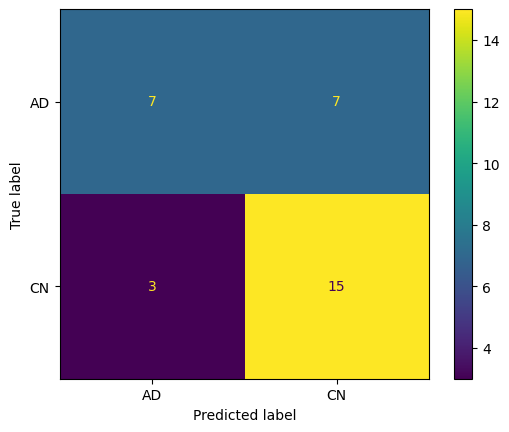
\includegraphics[width=\textwidth]{./imgs/resultados/axial/CN_AD_cm_AXIAL}
        \caption{Comparativa CN-AD. }
        \label{fig:mc-axial-cn-ad}
    \end{subfigure}
    \hspace*{\fill}
    \begin{subfigure}{0.45\textwidth}
        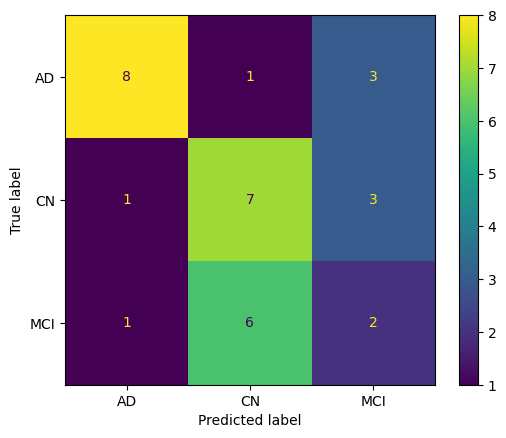
\includegraphics[width=\textwidth]{./imgs/resultados/axial/CN_MCI_AD_cm_AXIAL}
        \caption{Comparativa CN-MCI-AD. }
        \label{fig:mc-axial-cn-mci-ad}
    \end{subfigure}
    \caption{Matrices de confusión del plano Axial} \label{fig:mc-axial}
\end{figure}

Al comparar entre CN y AD en el plano axial se obtiene una precisión del 69\%
Frente al 53\% que se obtiene en la clasificación entre CN, MCI y AD. Además  en la comparación de dos clases se
observa un valor alto de falsos negativos.
En la clasificación de tres clases el etiquetado de la clase intermedia MCI ha sido  peor en comparación a CN y AD.


\subsection{Resultados del plano Coronal}\label{subsec:resultados-del-plano-coronal}

\begin{figure}[H]
    \centering
    \begin{subfigure}{0.45\textwidth}
        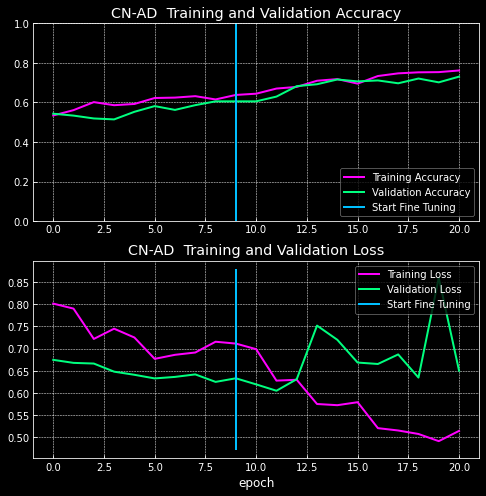
\includegraphics[width=\textwidth]{./imgs/resultados/coronal/CN_AD_output_CORONAL}
        \caption{Comparativa CN-AD. }
        \label{fig:coronal-cn-ad}
    \end{subfigure}
    \hspace*{\fill}
    \begin{subfigure}{0.45\textwidth}
        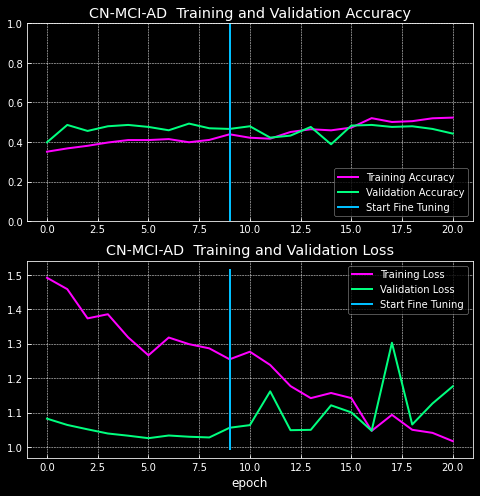
\includegraphics[width=\textwidth]{./imgs/resultados/coronal/CN_MCI_AD_output_CORONAL}
        \caption{Comparativa CN-MCI-AD. }
        \label{fig:coronal-c-mci-ad}
    \end{subfigure}
    \caption{Evolución del modelo durante el entrenamiento: plano Coronal.} \label{fig:coronal-model}
\end{figure}

\begin{table}[H]
    \centering
    \begin{tabular}{r r r r r}
        & precision & recall & f1-score & support \\
        AD & 0.83 & 0.59 & 0.69 & 17 \\
        CN & 0.65 & 0.87 & 0.74 & 15 \\
        & & & & \\
        accuracy &  &  & 0.72 & 32 \\
        macro avg & 0.74 & 0.73 & 0.72 & 32 \\
        weighted avg & 0.75 & 0.72 & 0.71 & 32 \\
    \end{tabular}
    \caption{Classification Report del plano Coronal. Comparativa CN-AD}
    \label{tab:cr-coronal-cn-ad}
\end{table}

\begin{table}[H]
    \centering
    \begin{tabular}{r r r r r}
        & precision & recall & f1-score & support \\
        AD & 0.67 & 0.50 & 0.57 & 8 \\
        CN & 0.62 & 0.50 & 0.56 & 10 \\
        MCI & 0.56 & 0.71 & 0.63 & 14 \\
        & & & & \\
        accuracy &  &  & 0.59 & 32 \\
        macro avg & 0.62 & 0.57 & 0.58 & 32 \\
        weighted avg & 0.61 & 0.59 & 0.59 & 32 \\
    \end{tabular}
    \caption{Classification Report del plano Coronal. Comparativa CN-MCI-AD}
    \label{tab:cr-coronal-cn-mci-ad}
\end{table}

\begin{figure}[H]
    \centering
    \begin{subfigure}{0.45\textwidth}
        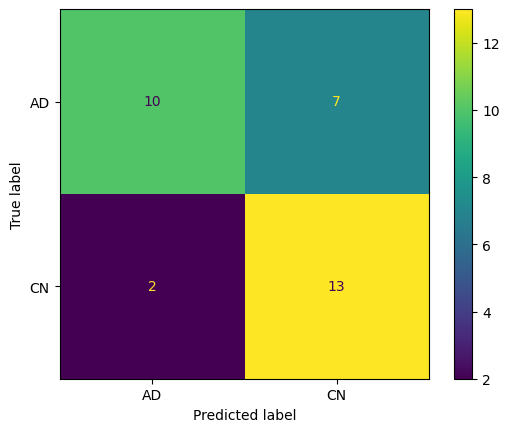
\includegraphics[width=\textwidth]{./imgs/resultados/coronal/CN_AD_cm_CORONAL}
        \caption{Comparativa CN-AD. }
        \label{fig:mc-coronal-cn-ad}
    \end{subfigure}
    \hspace*{\fill}
    \begin{subfigure}{0.45\textwidth}
        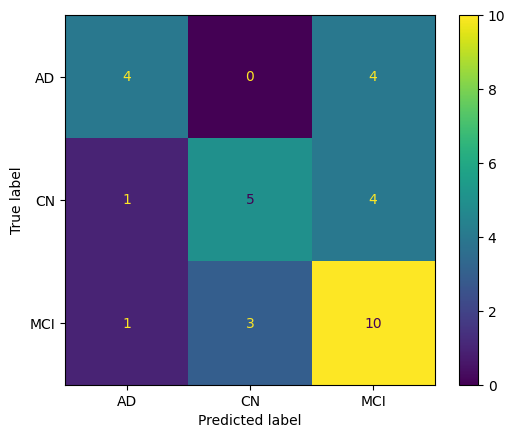
\includegraphics[width=\textwidth]{./imgs/resultados/coronal/CN_MCI_AD_cm_CORONAL}
        \caption{Comparativa CN-MCI-AD. }
        \label{fig:mc-coronal-cn-mci-ad}
    \end{subfigure}
    \caption{Matrices de confusión del plano Coronal.} \label{fig:mc-coronal}
\end{figure}

En una primera impresión, estos resultados son bastante buenos.
Al comparar entre CN y AD en el plano coronal se obtiene una precisión del 72\%, pero se observa que ha habido más
falsos negativos que falsos positivos.
En la clasificación entre CN, MCI y AD se obtiene una precisión del 59\% y un mayor número de falsos negativos, al
igual que en la clasificación de dos clases de este plano.

\subsection{Resultados del plano Sagital}\label{subsec:resultados-del-plano-sagital}

\begin{figure}[H]
    \centering
    \begin{subfigure}{0.45\textwidth}
        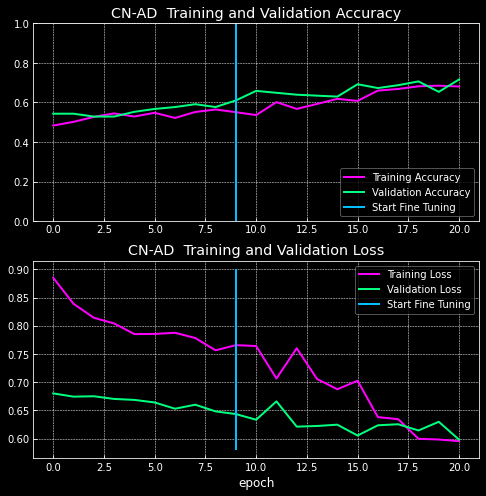
\includegraphics[width=\textwidth]{./imgs/resultados/sagittal/CN_AD_output_SAGITTAL}
        \caption{Comparativa CN-AD. }
        \label{fig:sagital-cn-ad}
    \end{subfigure}
    \hspace*{\fill}
    \begin{subfigure}{0.45\textwidth}
        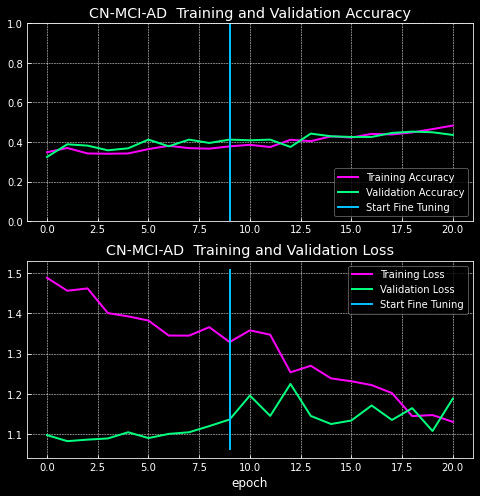
\includegraphics[width=\textwidth]{./imgs/resultados/sagittal/CN_MCI_AD_output_SAGITTAL}
        \caption{Comparativa CN-MCI-AD. }
        \label{fig:sagital-c-mci-ad}
    \end{subfigure}
    \caption{Evolución del modelo durante el entrenamiento: plano Sagital.} \label{fig:sagittal-model}
\end{figure}

\begin{table}[H]
    \centering
    \begin{tabular}{r r r r r}
        & precision & recall & f1-score & support \\
        AD & 0.64 & 0.67 & 0.65 & 21 \\
        CN & 0.30 & 0.27 & 0.29 & 11 \\
        & & & & \\
        accuracy &  &  & 0.53 & 32 \\
        macro avg & 0.47 & 0.47 & 0.47 & 32 \\
        weighted avg & 0.52 & 0.53 & 0.53 & 32 \\
    \end{tabular}
    \caption{Classification Report del plano Sagital. Comparativa CN-AD}
    \label{tab:cr-sagital-cn-ad}
\end{table}

\begin{table}[H]
    \centering
    \begin{tabular}{r r r r r}
        & precision & recall & f1-score & support \\
        AD & 0.48 & 0.62 & 0.54 & 16 \\
        CN & 1.00 & 0.10 & 0.18 & 10 \\
        MCI & 0.20 & 0.33 & 0.25 & 6 \\
        & & & & \\
        accuracy &  &  & 0.41 & 32 \\
        macro avg & 0.56 & 0.35 & 0.32 & 32 \\
        weighted avg & 0.59 & 0.41 & 0.37 & 32 \\
    \end{tabular}
    \caption{Classification Report del plano Sagital. Comparativa CN-MCI-AD}
    \label{tab:cr-sagital-cn-mci-ad}
\end{table}

\begin{figure}[H]
    \centering
    \begin{subfigure}{0.45\textwidth}
        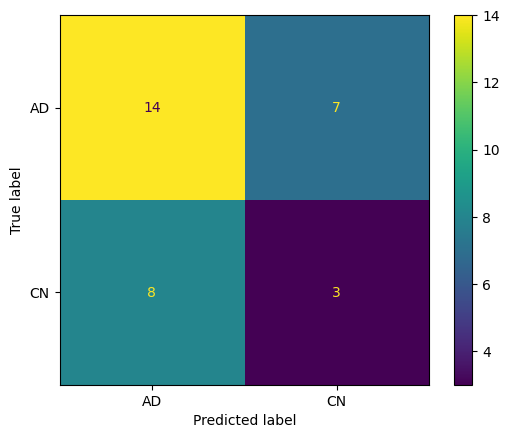
\includegraphics[width=\textwidth]{./imgs/resultados/sagittal/CN_AD_cm_SAGITTAL}
        \caption{Comparativa CN-AD. }
        \label{fig:mc-sagital-cn-ad}
    \end{subfigure}
    \hspace*{\fill}
    \begin{subfigure}{0.45\textwidth}
        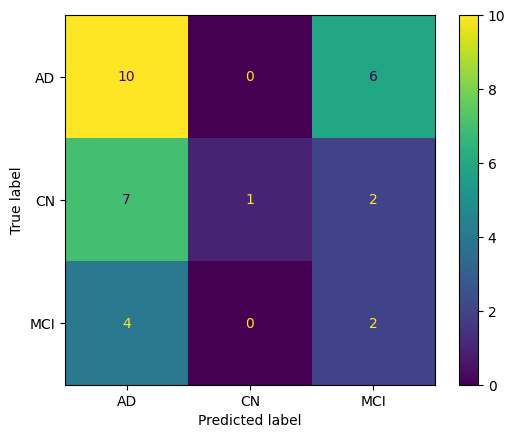
\includegraphics[width=\textwidth]{./imgs/resultados/sagittal/CN_MCI_AD_cm_SAGITTAL}
        \caption{Comparativa CN-MCI-AD. }
        \label{fig:mc-sagital-cn-mci-ad}
    \end{subfigure}
    \caption{Matrices de confusión del plano Sagital.} \label{fig:mc-sagittal}
\end{figure}

En el plano sagital se obtiene una precisión del 53\% en la clasificación entre CN y AD y un 40\% en la clasificación
entre CN, MCI y AD. Destacan en ambos una tendencia a etiquetar con más facilidad el tipo AD dando lugar a un mayor
número de falsos positivos que de falsos negativos.

\section{Conclusión}\label{sec:conclusion}

Para empezar hay que concluir que la evolución de los modelos durante el entrenamiento es muy similar.
En ninguno de los casos se obtiene una precisión mayor al 80\%.
Y además la tendencia de la función de pérdida es un indicador de que quizás haría falta un mayor número de muestras de
entrenamiento.
En este caso hemos utilizado el mayor número posible de las disponibles creando un dataset balanceado.
Sería interesante plantear una nueva vertiente en la que se mezclen biomarcadores de varias fuentes de datos como hacen
algunos estudios de la literatura, y como también se intentó en un principio en este proyecto, pero los requerimientos
de acceso a tales repositorios de datos es otro impedimento.

En cuanto a la pregunta que marca el objetivo de este proyecto. \textbf{¿Qué plano es mejor para el diagnóstico del
Alzheimer?} Claramente, teniendo en mente el valor de la precisión, en el \textbf{plano coronal} un mayor porcentaje
de datos han sido etiquetados de forma correcta que en el resto de planos tanto en la comparativa de 2 clases como
en la comparativa de 3 clases.

Además el plano coronal anatómicamente engloba las tres regiones más importantes del cerebro relacionadas con la EA:
el hipocampo, la corteza y los ventrículos.
Por lo tanto, con los datos que se han obtenido se puede concluir que sí es el mejor plano para el diagnóstico de la
enfermedad.

Además, con este sistema se podrían integrar los tres los tres modelos de manera que, una vez que se ha realizado
la clasificación usando cada plano, realizar un diagnóstico por votación siendo el resultado final el más votado de la
unión de los resultados de los tres modelos.


    \chapter{Aplicación web para el diagnóstico del Alzheimer mediante MRI}
\label{ch:aplicacion-web-para-el-diagnostico-del-alzheimer-mediante-mri}
Como segundo objetivo de este proyecto se plantea poder aplicar el estudio realizado en un ejemplo real, en este caso
en una aplicación web.
En este capítulo se detalla el proceso que se ha seguido hasta completarla.
Siguiendo la metodología comentada en la sección~\ref{sec:metodologia-herramientas-y-obstaculos}.

\section{Especificación del sistema}\label{sec:especificacion-del-sistema}
Para poder completar una especificación del sistema es necesario conocer las necesidades de los usuarios, por lo que se
han creado 2 usuarios ficticios que darán forma a la HU que detalla el sistema.

\subsection{Usuarios}\label{subsec:usuarios}
\begin{table}[H]
    \centering
    \begin{tabular}{| l | l|}
        \hline
        Nombre & Blanca \\
        \hline
        Edad & 22 años \\
        \hline
        Ocupación & Estudiante de radiología \\
        \hline
        Personalidad & Extrovertida y analítica \\
        \hline
        Metas & Conseguir especializarse en el campo de radiología \\
        \hline
        Habilidades tecnológicas & Altas \\
        \hline
    \end{tabular}
    \caption{Usuarios ficticios: Persona 1}
    \label{tab:persona1}
\end{table}

\begin{table}[H]
    \centering
    \begin{tabular}{| l | l|}
        \hline
        Nombre & Ana \\
        \hline
        Edad & 45 años \\
        \hline
        Ocupación & Experta en radiología \\
        \hline
        Personalidad & Sensible y positiva \\
        \hline
        Metas & Poder mejorar el área de radiología del centro en el que trabaja \\
        \hline
        Habilidades tecnológicas & Altas \\
        \hline
    \end{tabular}
    \caption{Usuarios ficticios: Persona 2}
    \label{tab:persona2}
\end{table}


Blanca y Ana tienen un alto conocimiento teórico en este ámbito, forman parte de este estudio que se está realizando,
son futuras usuarias de la aplicación y participan como clientes de la misma realizando la historia de usuario que
define la especificación del sistema.

\subsection{Historia de Usuario}\label{subsec:historia-de-usuario}
La HU que se define es la siguiente:

\textbf{Como profesional de entornos clínicos quiero poder conocer el grado de Enfermedad de Alzheimer en una resonancia
magnética de manera sencilla.}

\begin{itemize}
    \item \textbf{Descripción}: Como usuario, quiero poder conocer cuál es el grado de enfermedad de Alzheimer presente
    en una neuroimagen, en concreto en una MRI de tipo \textit{NIfTI}.
    Con el objetivo de realizar un diagnóstico de enfermedad de Alzheimer sin necesidad de instalar ningún programa
    software para visualizar imágenes cerebrales
    \item \textbf{Pruebas de Aceptación del Usuario}: Subir un archivo \textit{NIfTI} y obtener una clasificación de la
    imagen y el valor del grado presente correspondiente en términos de Enfermedad de Alzheimer.

\end{itemize}

De esta necesidad surge \textbf{Alz Care}.

\textbf{Alz Care} se idea para ser una aplicación que una Inteligencia Artificial y salud.
En ella a partir de Imágenes por resonancia magnética se obtiene una clasificación del deterioro cognitivo y EA presentes.


\section{Proceso de Diseño}\label{sec:proceso-de-diseno}
En esta sección se muestra el proceso de diseño llevado a cabo para \textbf{Alz Care}, así como su identidad visual y
prototipos.

\subsection{Identidad visual}\label{subsec:identidad-visual}

\subsubsection{Paleta de colores}

La paleta de colores elegida es la siguiente:

\begin{figure}[H]
    \centering
    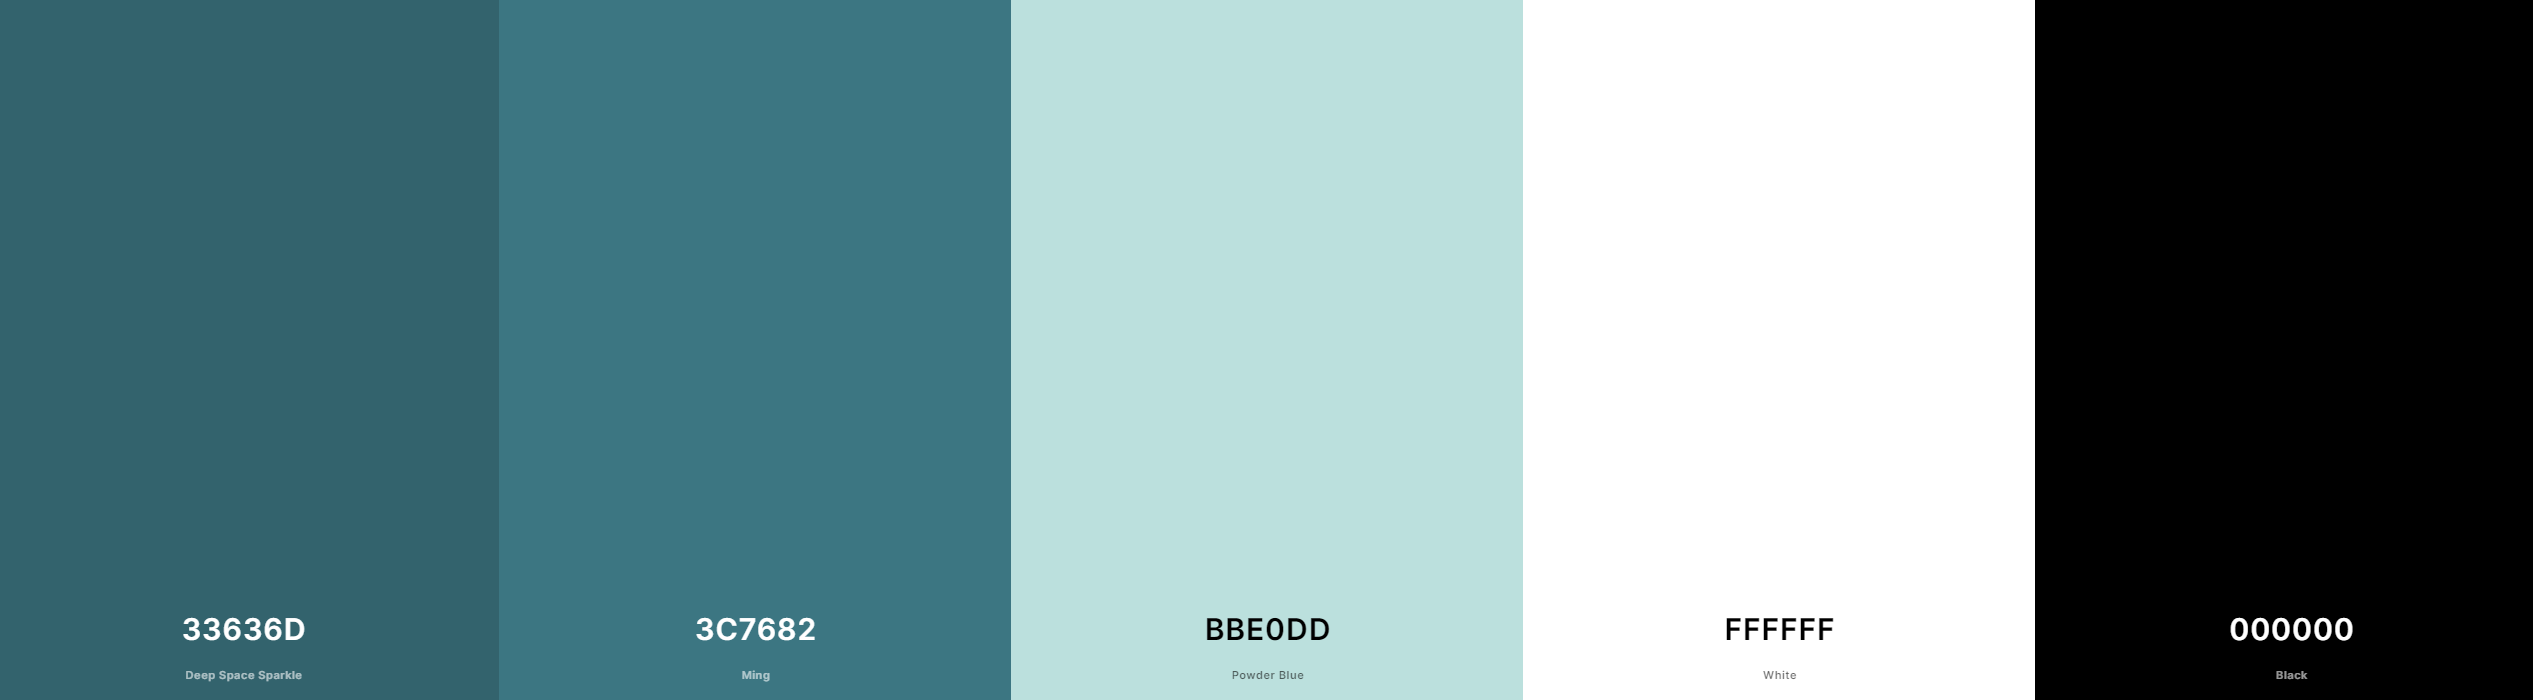
\includegraphics[width=\textwidth]{./imgs/app/paleta}
    \caption{Paleta de colores de Alz Care}
    \label{fig:paleta-colores}
\end{figure}

Se elige esta paleta porque se busca minimalismo y serenidad y el uso de tonos verdes azulados para mantener una
relación con el mundo de la salud.

\subsubsection{Logotipo}

El logotipo de la aplicación se ha realizado usando la herramienta
Paint3D~\footnote{~\cite{paint-3d}{Paint3D}}.

\begin{figure}[H]
    \centering
    
\includegraphics[width=\textwidth]{./imgs/app/icon-name}
    \caption{Logotipo de Alz Care}
    \label{fig:logotipo}
\end{figure}

\subsection{Mockup: UI UX Design}\label{subsec:mockup:-ui-ux-design}
Para facilitar el desarrollo de la misma, se ha realizado un prototipo de las páginas principales.
Se ha hecho uso de Figma~\footnote{~\cite{figma}{Figma}} como herramienta de generación de prototipos.
Las vistas generadas son las siguientes:

\begin{figure}[H]
    \centering
    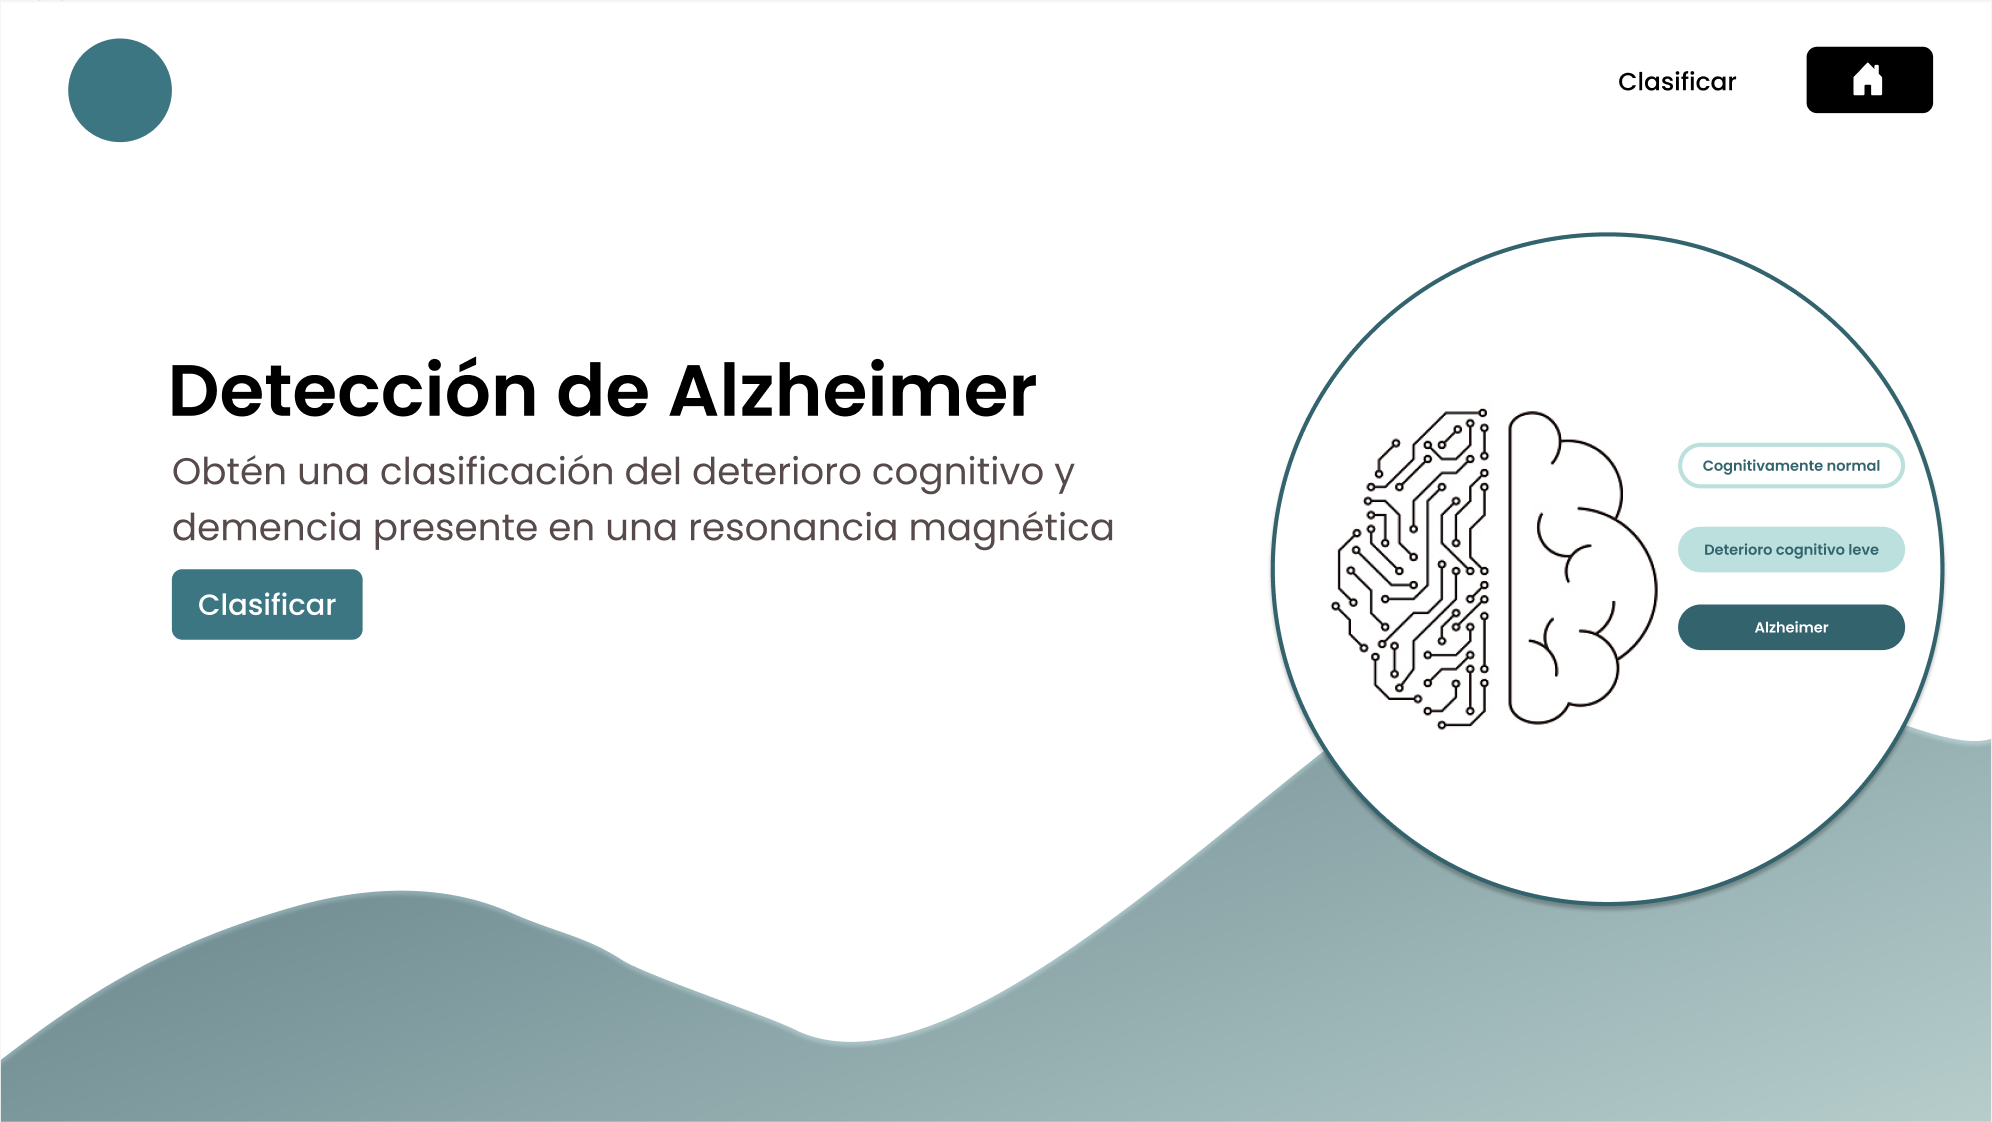
\includegraphics[width=\textwidth]{./imgs/app/landing-page}
    \caption{Landing Page}
    \label{fig:landing-page}
\end{figure}

\begin{figure}[H]
    \centering
    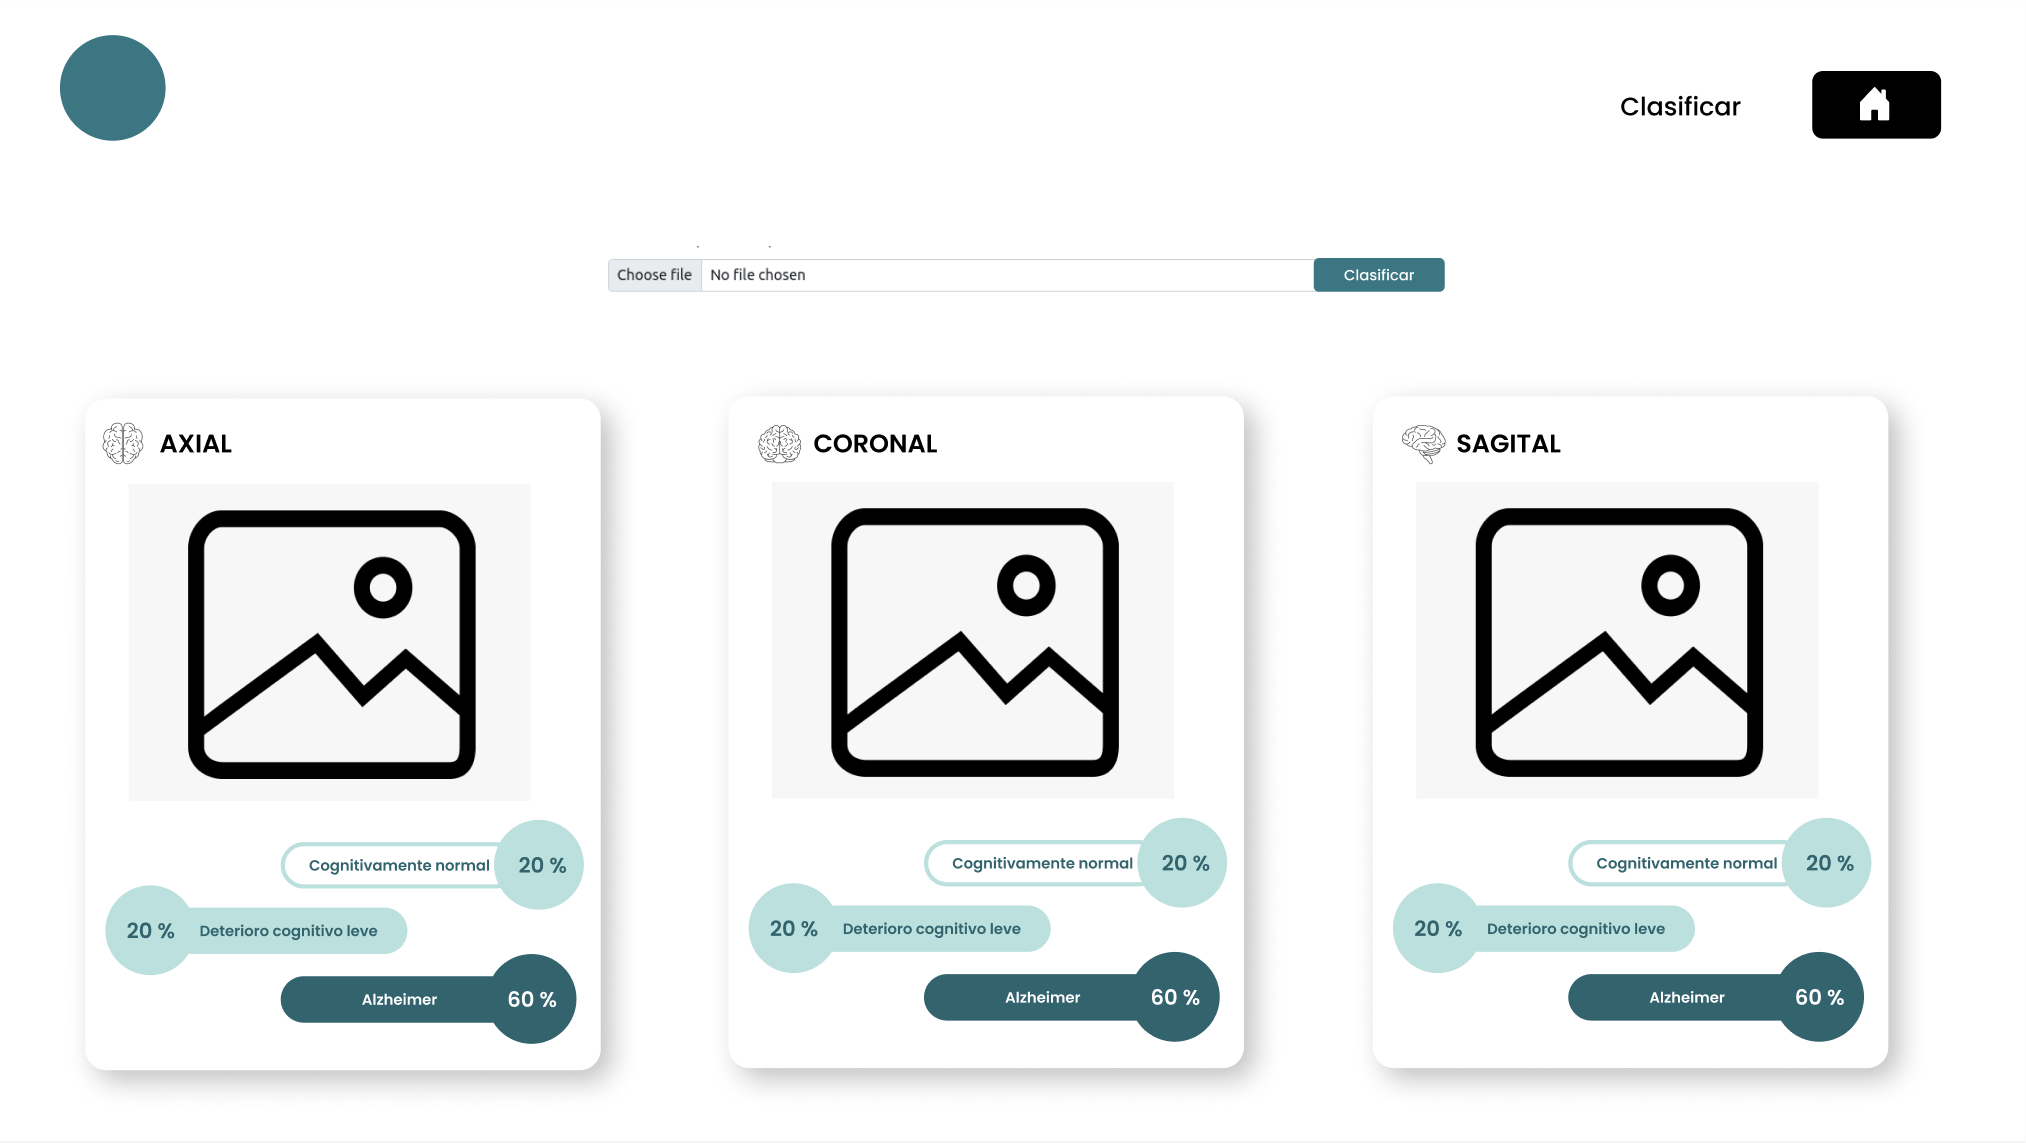
\includegraphics[width=\textwidth]{./imgs/app/vista-clasificacion}
    \caption{Vista De Clasificación}
    \label{fig:vista-clasificacion}
\end{figure}

\section{Implementación}\label{sec:implementacion}
Para la implementación de \textbf{Alz Care} se ha decidido usar una arquitectura
\textit{cliente-servidor}~\footnote{~\cite{cliente-servidor}{Modelo de comunicación  cliente-servidor}}, facilitando
así la utilización de la parte del servidor por otras aplicaciones o servicios de cara a posteriores trabajos.

En el lado del servidor o backend es donde se encuentra la lógica de la aplicación y donde se va a realizar la
integración con el sistema de aprendizaje profundo.
Se mantiene como lenguaje de programación Python, para poder seguir haciendo uso de las librerías necesarias para el
procesamiento de biomarcadores MRI de tipo NIfTI y las herramientas para trabajar con el sistema de DL.

Como framework se ha utilizado \textbf{flask-smorest}, una librería framework para crear API REST de la mano de
\textbf{Flask}, que es un genial candidato para desarrollar API en Python de manera ágil que dispone de un depurador
y soporte integrado para pruebas unitarias.
Además como herramienta de validación de datos se utiliza \textbf{marshmallow} y para la documentación de la API se utiliza
\textbf{Swagger}.

Para la gestión de dependencias se utiliza \textbf{Poetry}, ya que es una herramienta gestiona las bibliotecas de las que depende
tu proyecto por ti.
Evitando errores entre versiones y facilitando la creación del entorno de trabajo.

Del lado del cliente se ha utilizado \textbf{React} por ser una librería muy completa con la que crear interfaces de usuario
mediante componentes de manera sencilla.
Y que dispone de un amplio abanico de librerías externas, como \textbf{Framer Motion}, una biblioteca de animación que ha
facilitado la integración de animaciones mejorando la experiencia de usuario de la aplicación.

Como parte de la metodología de trabajo, se han incluido como Integración Continua dos pipelines para el código al
proyecto en \textit{GitHub} Actions para asegurar la integridad de la aplicación a la incorporación de nuevas funcionalidades.
Se ha incorporado uno para el backend y otro para el frontend, en ambos se persigue la misma meta: evitar errores en
el código fuente, mediante flake8 para el servidor y prettier para el frontend, y la ejecución de tests.


\section{Resultados}\label{sec:resultados}

En esta sección se muestra el resultado final de la vista de la aplicación.

Tal y como se puede ver, el objetivo es presentar una aplicación que sea clara y con la que los usuarios se lleven una
buena experiencia de uso.

Para ello tal y como se ve en la Figura~\ref{fig:home-page}, la página de inicio o \textit{landing page} muestra una vista
general de la funcionalidad principal de la aplicación.
En ella se ve claramente qué se va a obtener con la aplicación gracias a la descripción principal que aparece.

En la Figura~\ref{fig:final-cp-page} se muestra la página de clasificación.
Es una página muy simple de la que se espera que el usuario reaccione de manera directa con el formulario para subir
una imagen.
Como futura mejora se propone que el icono de fondo sea una imagen en tonos neutros que muestre los pasos que hay que
realizar.

Como hay una restricción en cuanto al tipo de archivo que se puede subir, en caso de tipo de archivo incorrecto o no
válido se muestra el mensaje por pantalla: Figura~\ref{fig:final-cp-error-page}.
De la misma forma, si hubiera algún tipo de error con la conexión del servidor también muestra error.

En la Figura~\ref{fig:final-cp-r-page} se muestra la página más relevante.
En ella, tras haberse completado la petición al servidor y haber obtenido respuesta.
Se muestra una \textit{card} o \textit{tarjeta} por cada plano de la MRI con su correspondiente clasificación de
deterioro cognitivo, mostrando el porcentaje asociado al valor que devuelve el modelo.
Cada tarjeta contiene como título el plano asociado y un icono del plano.
Si bien es cierto que los usuarios de la aplicación son personas de entornos clínicos que entienden de la materia,
le aporta información y valor a la vista.

Esta vista presenta también muchas ventajas y es que sin necesidad de instalar ningún software visor de biomarcadores
MRI se han podido visualizar los tres cortes más importantes de la MRI.

Además, en este documento solo se muestran imágenes, pero se han añadido animaciones mejorando la experiencia de usuario.

\begin{figure}[H]
    \centering
    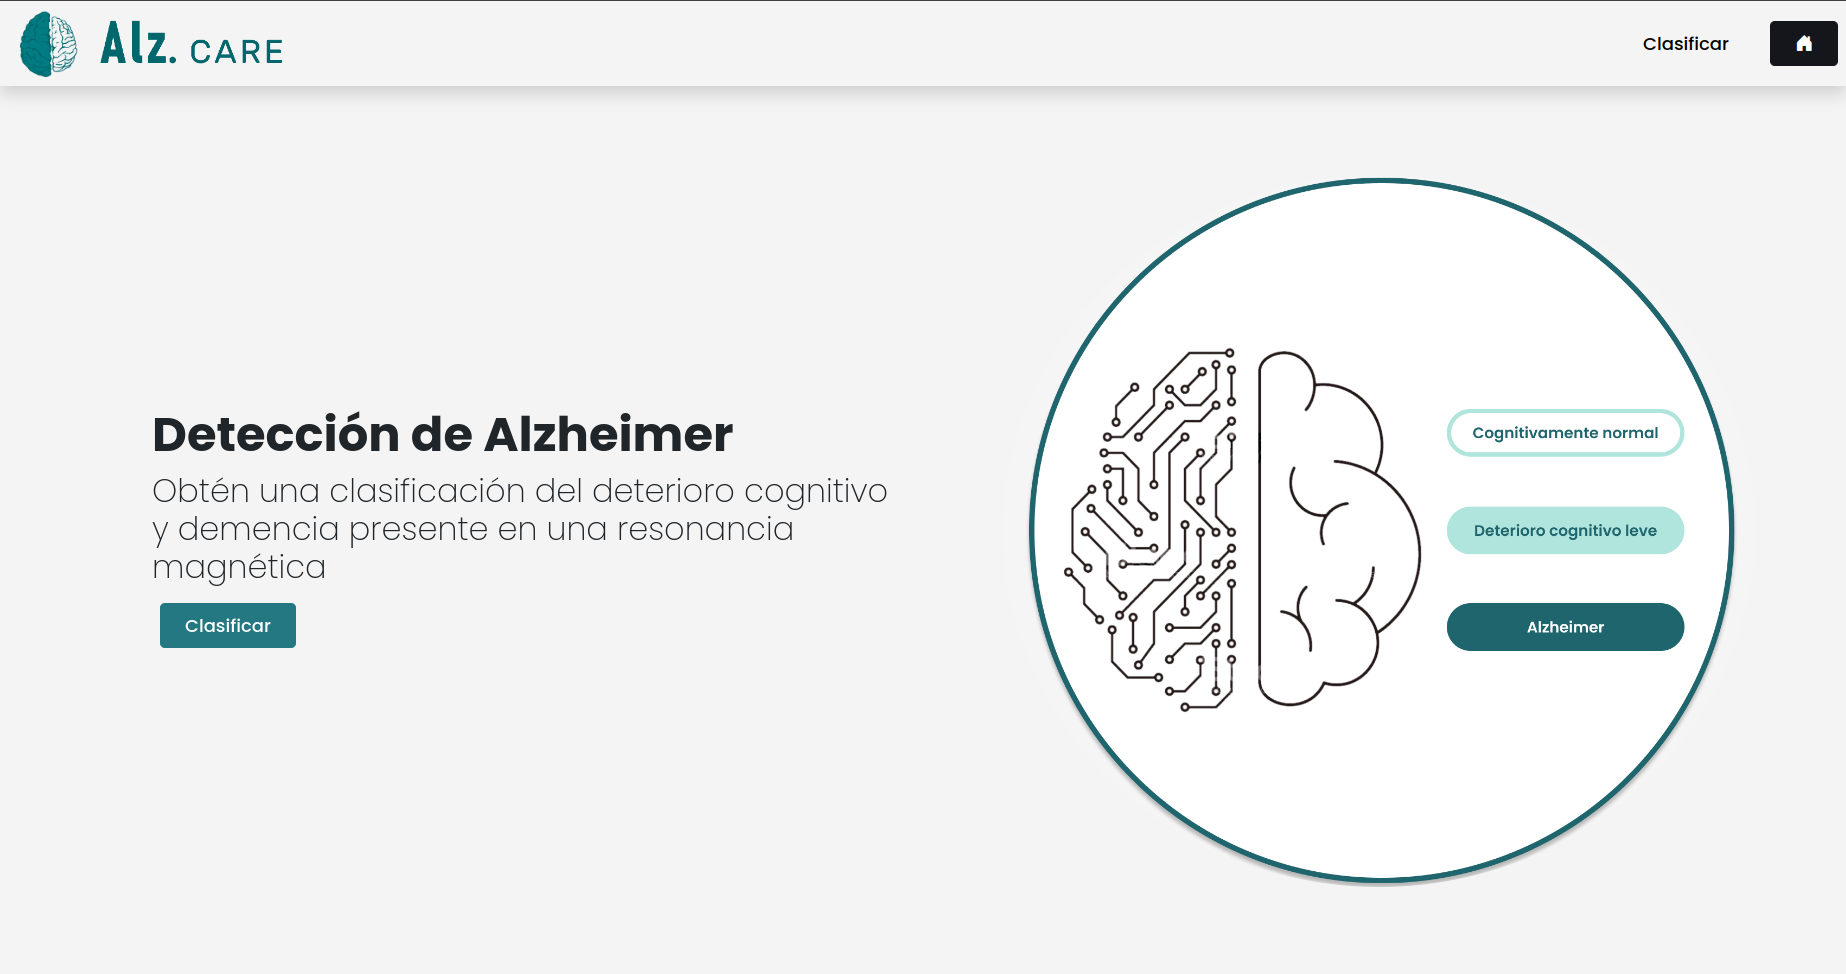
\includegraphics[width=\textwidth]{./imgs/app/final-home}
    \caption{Home Page de Alz Care}
    \label{fig:home-page}
\end{figure}

\begin{figure}[H]
    \centering
    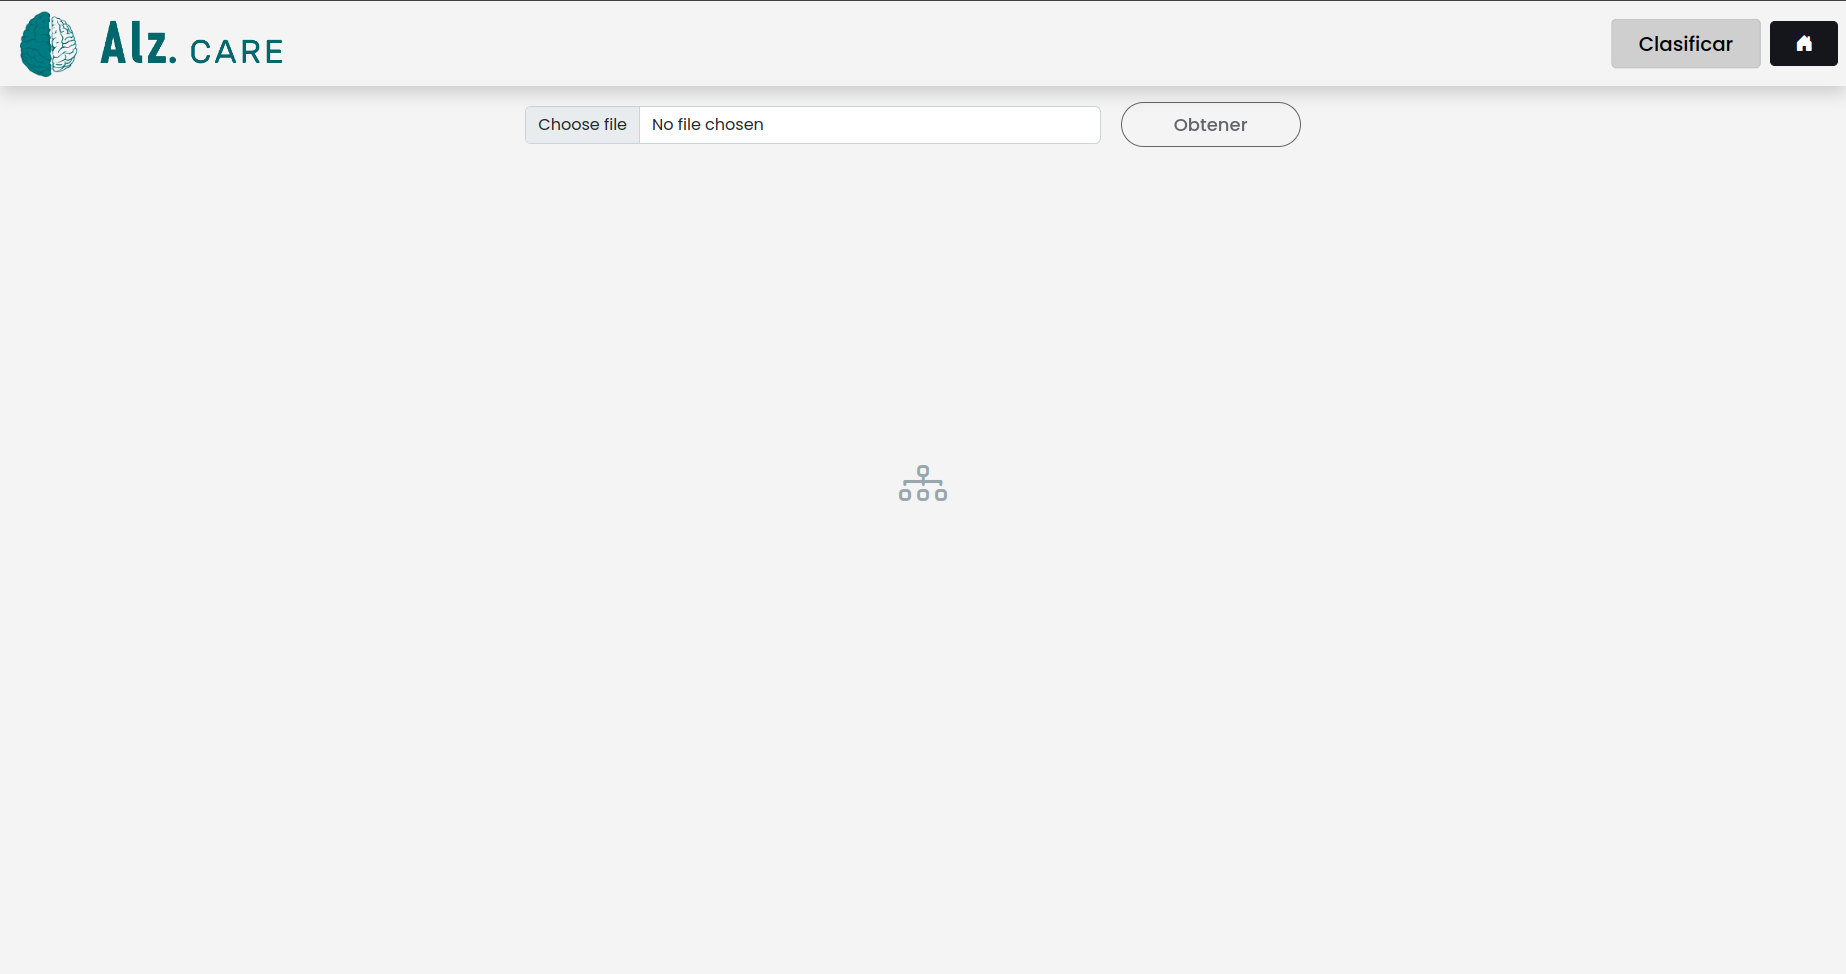
\includegraphics[width=\textwidth]{./imgs/app/final-cp}
    \caption{Vista De Clasificación de Alz Care}
    \label{fig:final-cp-page}
\end{figure}

\begin{figure}[H]
    \centering
    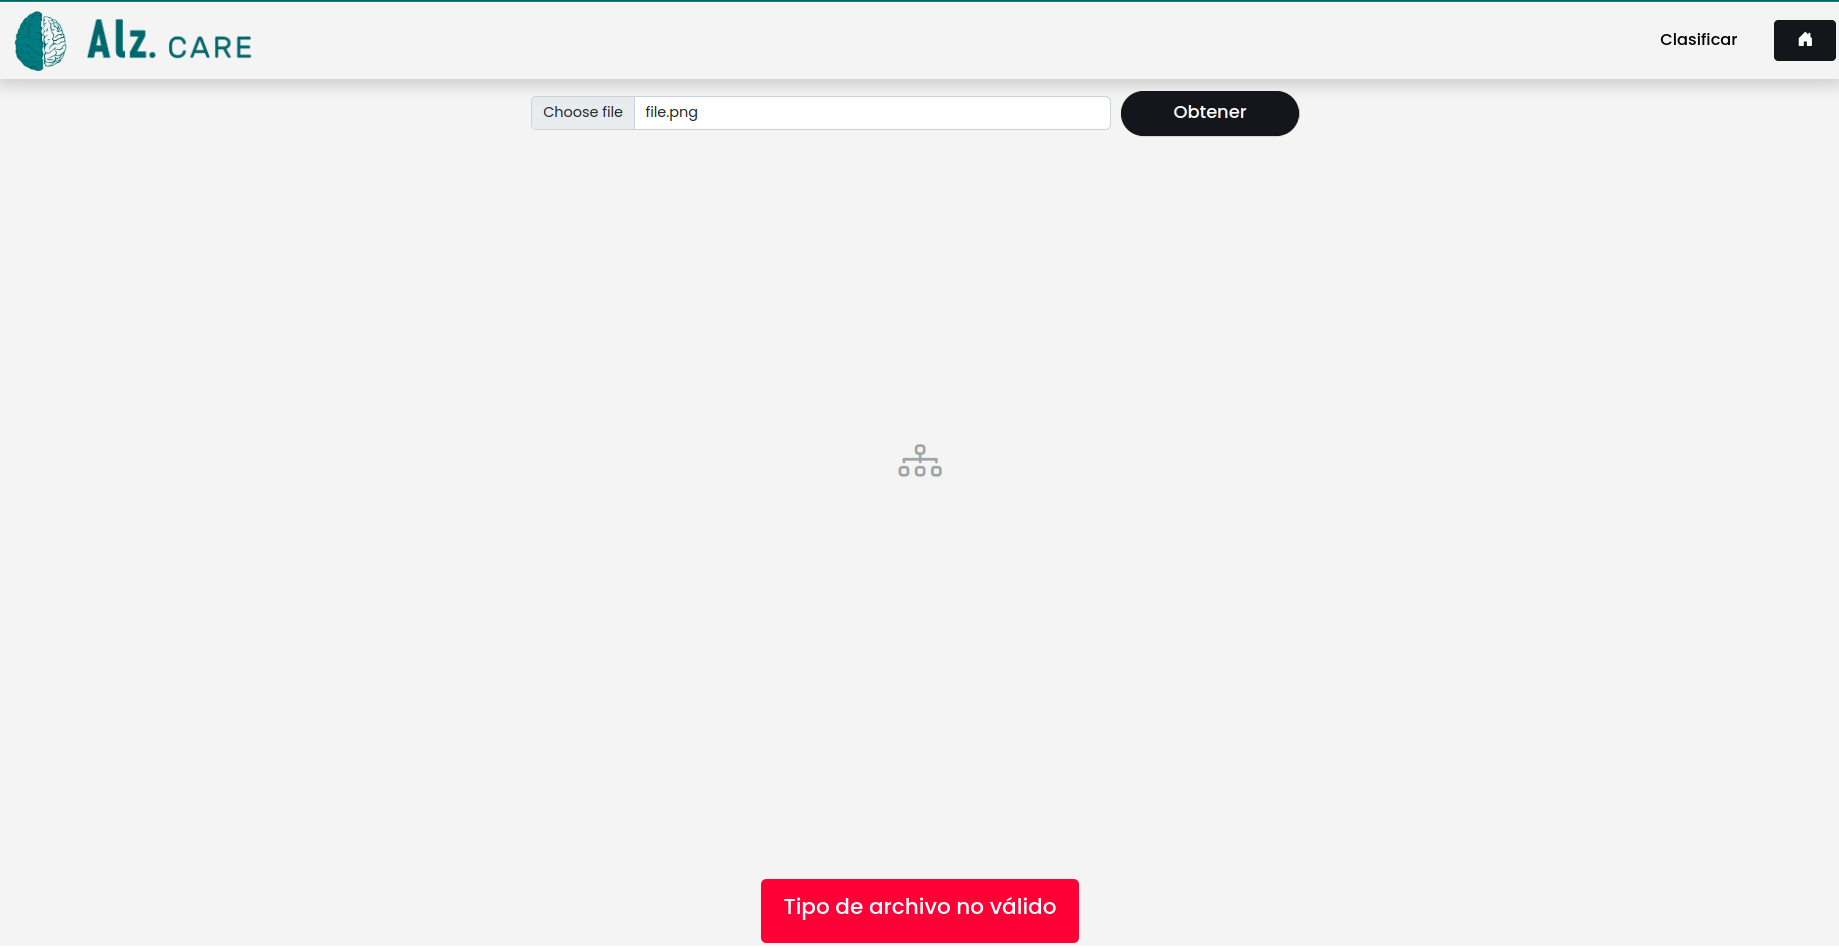
\includegraphics[width=\textwidth]{./imgs/app/final-cp-error}
    \caption{Vista De Clasificación de Alz Care: Tipo de archivo no válido}
    \label{fig:final-cp-error-page}
\end{figure}

\begin{figure}[H]
    \centering
    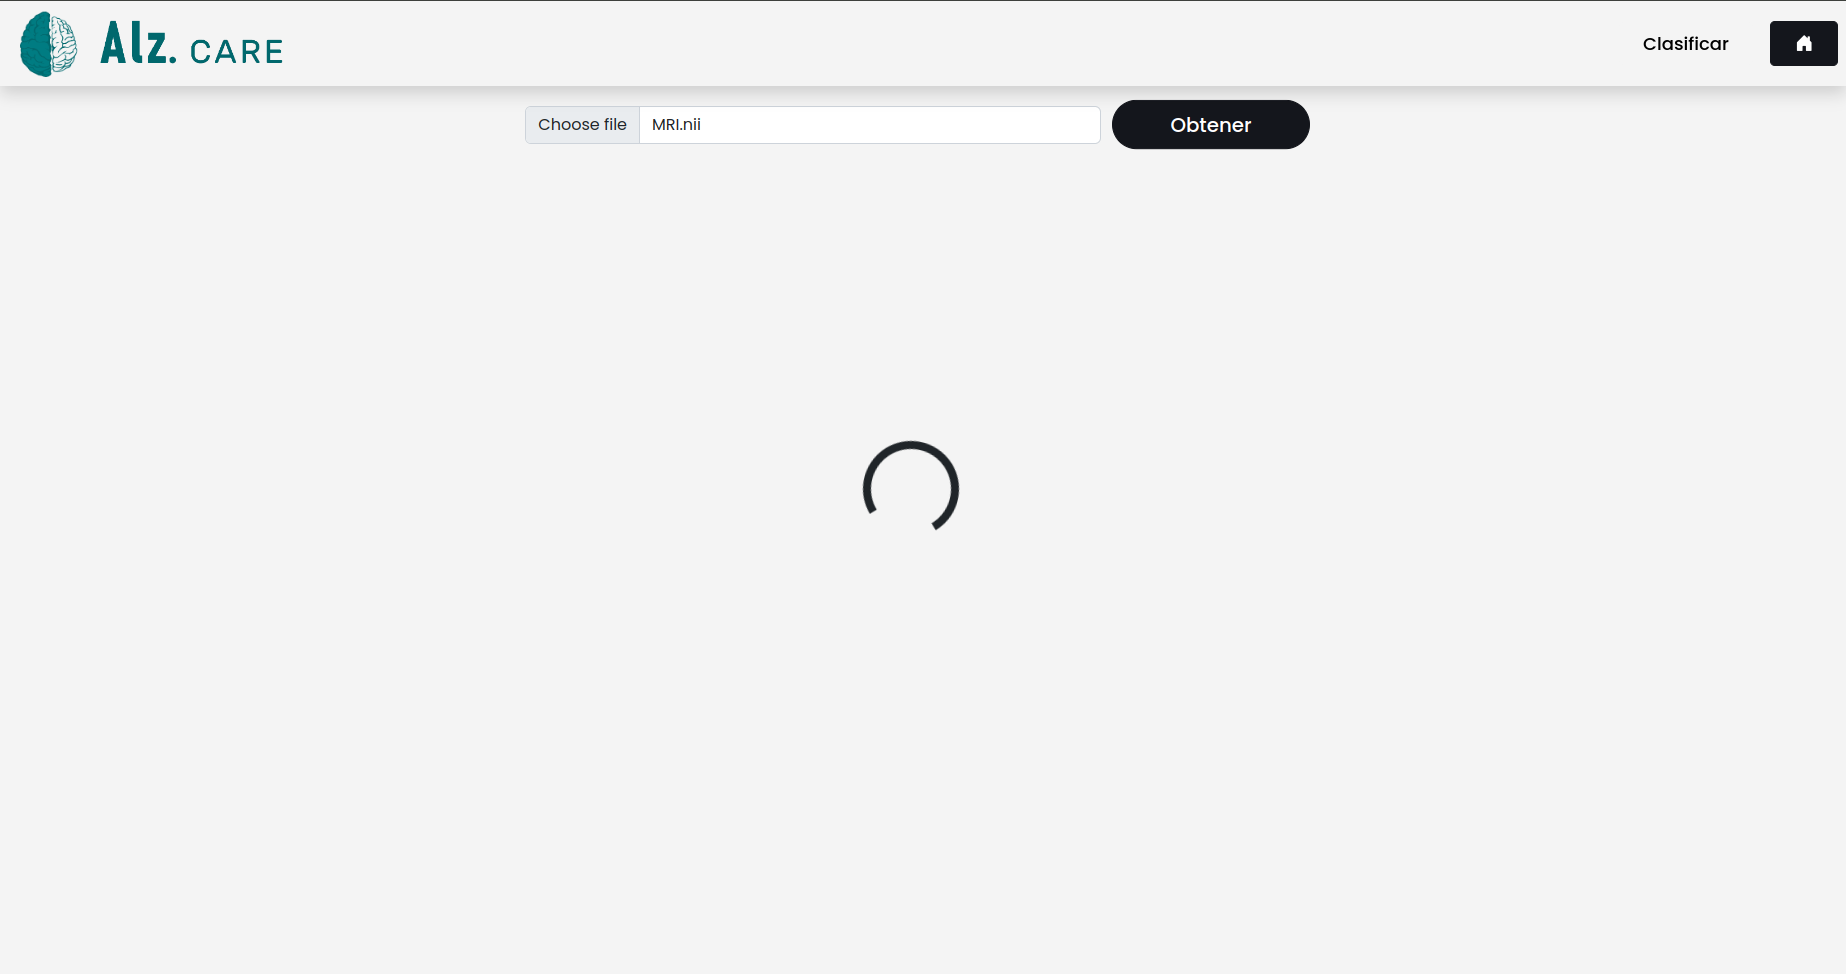
\includegraphics[width=\textwidth]{./imgs/app/final-cp-l}
    \caption{Vista De Clasificación de Alz Care: Cargando datos}
    \label{fig:final-cp-l-page}
\end{figure}

\begin{figure}[H]
    \centering
    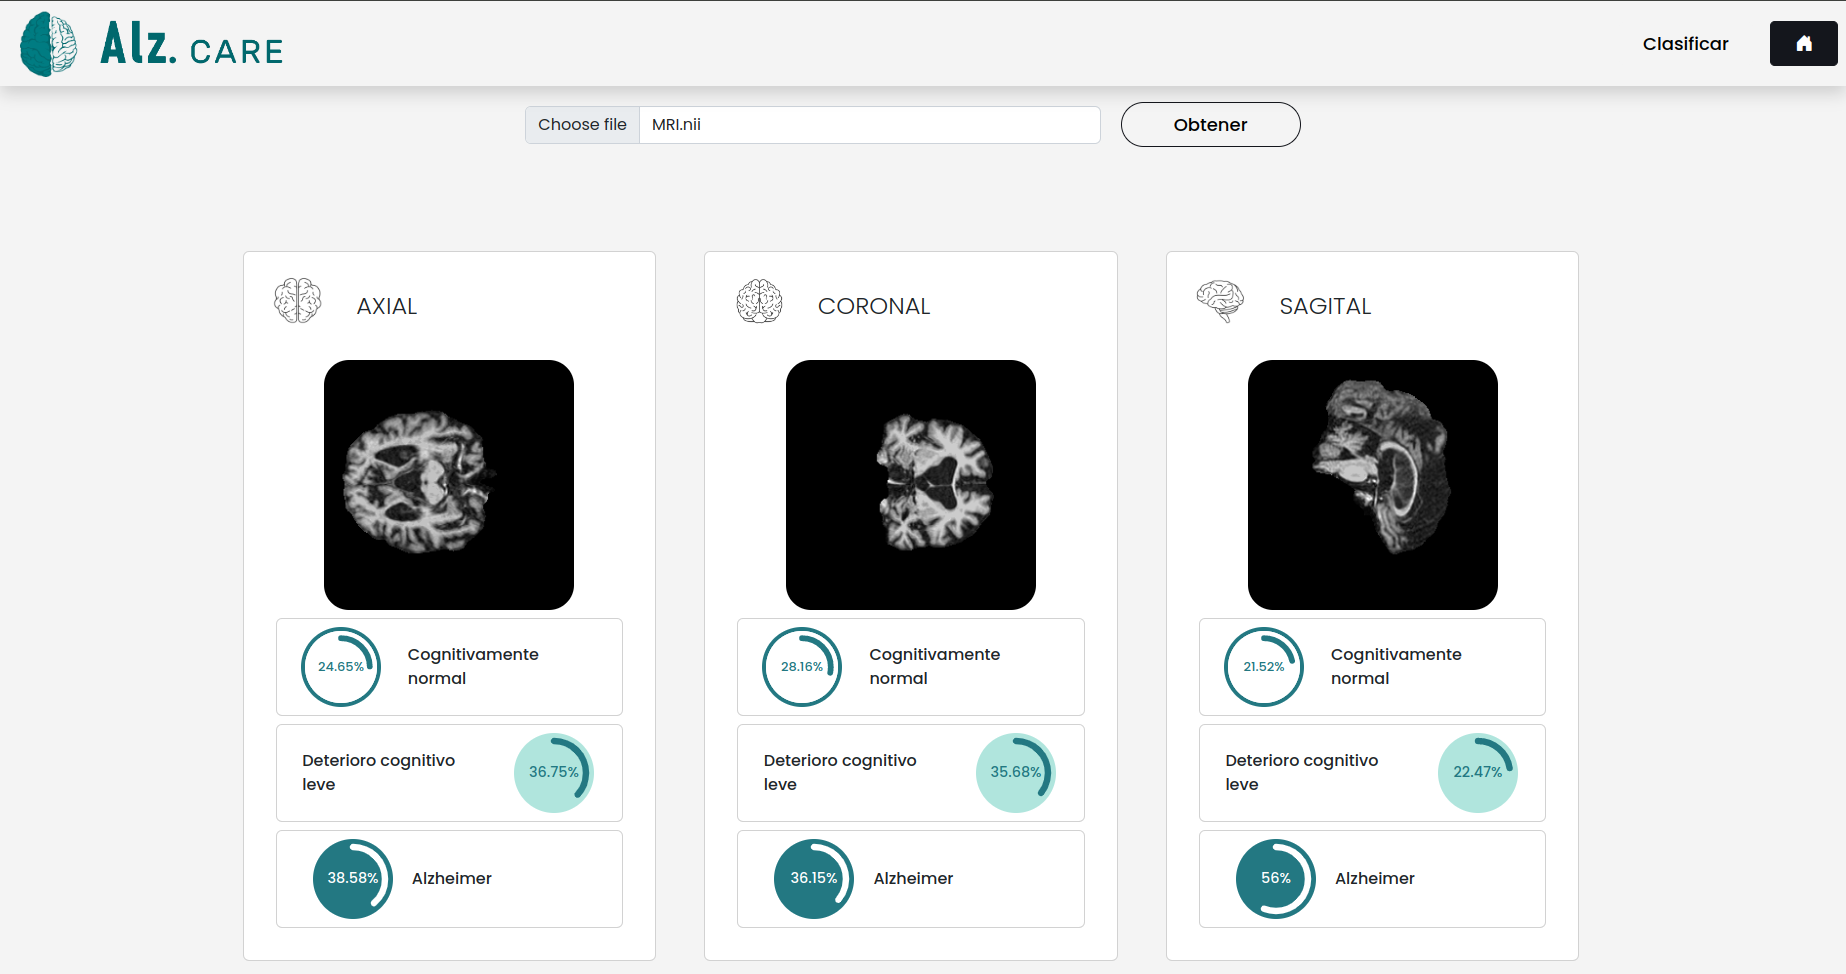
\includegraphics[width=\textwidth]{./imgs/app/final-cp-r}
    \caption{Vista De Clasificación de Alz Care: Resultados}
    \label{fig:final-cp-r-page}
\end{figure}


    \chapter{Conclusiones y Trabajos Futuros}\label{ch:conclusiones-y-trabajos-futuros}

\section{Conclusiones}\label{sec:conclusiones}
Con este proyecto se pretendía realizar un estudio de técnicas de DL para el diagnóstico de la EA.
En concreto se centró el objetivo general del estudio en identificar con qué plano cerebral se obtiene mejor rendimiento
a partir de biomarcadores de tipo MRI. En la literatura actual no quedaba bien definido qué plano era mejor.

Tras realizar un análisis de la base de datos se observó que el conjunto de datos disponible era limitado y no estaba
balanceado por lo que se ha balanceado y realizado la extracción de imágenes de 2D de los biomarcadores MRI de 3D,
generando los datasets de entrenamiento correspondientes a los casos de análisis.
Añadiendo también una comparación entre la clasificación de imágenes usando 2 clases, CN y AD, y usando 3 clases, CN,
MCI y AD, de manera que se realiza un estudio más en profundidad de estas técnicas para la medición del deterioro
cognitivo.

Los resultados muestran que una clasificación mediante 2 clases proporciona mucho mejor rendimiento que la clasificación
mediante 3 clases, sucediendo con esta tendencia para todas las vistas cerebrales y que se debe fundamentalmente a que
el conjunto de datos es reducido.

En cuanto a la pregunta final, sobre qué plano es mejor, al utilizarse el mismo conjunto de biomarcadores para la
extracción de los cortes 2D, queda demostrado que el plano coronal es el mejor de los 3, con un rendimiento del 72\%
frente al 69\% del plano axial y el 53\% del plano sagital.

Además, teniendo en cuenta que el plano coronal engloba las tres regiones más importantes del cerebro relacionadas con
la EA como son el hipocampo, la corteza y los ventrículos.
Se concluye que los resultados son acordes a lo esperado.
Pudiendo servir como guía para futuras conclusiones en esta área de investigación.

Por otra parte también se buscaba facilitar el uso de estas técnicas en una aplicación real.
De lo cual surge Alz Care, una pequeña aplicación que integra un sistema DL, en este caso el
previamente obtenido en el desarrollo experimental, pero que puede ser escalable a otros modelos.
Esta aplicación permite al usuario conocer el grado de deterioro cognitivo de una RMI ,y la visualización
de los planos incluidos en la misma, de una manera sencilla y sin tener que instalar ninguna herramienta de
visualización o programa externo.

Pudiendo resultar de gran utilidad en la labor de los médicos o personas de entornos clínicos que tengan este tipo de
necesidades.


\section{Trabajos Futuros}\label{sec:trabajos-futuros}
Con este TFG se obtiene respuesta a las preguntas iniciales, pero con un rendimiento que podría mejorarse con la
utilización de un mayor conjunto de datos.
Como podría ser combinando los biomarcadores de múltiples bases de datos o probando otras técnicas o arquitecturas.

En cuánto a la aplicación web, se ha considerado como un mínimo producto viable.
Sería interesante ampliarla y para ello se establecen tres ideas o puntos de partida que no ha sido posible incluir en
este proyecto por la extensión del mismo.
Las tres ideas que se proponen son:
\begin{itemize}
    \item Ampliar la lógica para que se utilice como aplicación de gestión de paciente de EA en la que se incluya un
    modelo que clasifique más clases y, por lo tanto, pueda servir como seguimiento de la enfermedad.
    \item Agrandar el diagrama arquitectónico de la solución y formar una aplicación que integre más enfermedades y más
    sistemas de clasificación.
    \item Incluir un visualizador completo de RMI en línea.
\end{itemize}


    \newpage
    \appendix\addcontentsline{toc}{chapter}{Apéndices}
    \chapter{ADNI}\label{ch:aped.a}
\textbf{Alzheimer’s Disease Neuroimaging Initiative (ADNI)\footnote{\href{https://adni.loni.usc.edu/}{ADNI}}} es un
estudio longitudinal multicéntrico en el que se desarrollan biomarcadores genéticos, bioquímicos y de imagen para la
detección temprana y el seguimiento de la enfermedad de Alzheimer, y que tiene como objetivos principales:
\begin{itemize}
    \item La detección de la EA en la fase más temprana posible y determinar procedimientos para hacer un seguimiento
    de la enfermedad con biomarcadores.
    \item Apoyar los avances en la intervención, prevención y tratamiento de la EA mediante el uso de nuevos métodos de
    diagnóstico en las etapas más tempranas posible, actuando así en el momento en el que la intervención puede ser más eficaz.
    \item Contribuir en la investigación de la EA, proporcionando los datos entre investigadores de todo el mundo.\\
\end{itemize}

Los datos utilizados en este TFG se han obtenido de esta base de datos.
Su acceso es gratuito, pero es necesario realizar una solicitud en la que se indica el motivo por el que se requiere el
acceso a los datos de ADNI, la afiliación institucional a la que se pertenece como investigador, y posteriormente
obtener una aprobación de la solicitud.
Además implícitamente se acepta un acuerdo de uso de datos, ya que estos datos no pueden ser utilizados con fines comerciales.

Al solicitar el acceso se puede hacer la solicitud a tres estudios diferentes: ADNI,
AIBL\footnote{\href{https://aibl.csiro.au/}{AIBL}} y DOD-ADNI. Cada estudio tiene su propio acuerdo de uso de datos.
En cuanto al mantenimiento de la cuenta, se requiere de la presentación de una actualización anual, en caso contrario,
la cuenta expirará automáticamente (se envía previamente un recordatorio por correo electrónico).

ADNI comenzó en 2004 bajo la dirección del \textit{Dr. Michael W. Weiner}, obteniendo financiación para un estudio
inicial de 5 años: ADNI-1 con el objetivo de desarrollar biomarcadores como medidas de resultado para ensayos clínicos,
el cual se amplió varias veces, la primera en 2009 dando lugar a ADNI-GO (Grand Opportunities) con el propósito de
examinar los biomarcadores en las primeras fases de la enfermedad, y la segunda y tercera ampliación en 2011 y 2016 con
ADNI-2 y ADNI-3 para el desarrollo de biomarcadores como predictores del deterioro cognitivo y para el estudio del uso
de PET de tau y técnicas de imagen funcional en ensayos técnicos respectivamente.

ADNI incluye participantes de entre 50 y 90 años de edad de Estados Unidos y Canadá, que se someten a una serie de
pruebas iniciales que se repiten en intervalos en los posteriores cuatro años.
El mayor número de participantes se encuentra en la franja de 70 a 79 años.
Se dividen en distintos grupos de investigación según el grado de enfermedad de Alzheimer presente,desde individuos
sanos, pacientes con deterioro cognitivo leve hasta pacientes que padecen EA.

Los datos de ADNI están administrados por LONI\footnote{\href{https://loni.usc.edu/}{LONI}} a partir de
IDA\footnote{\href{https://ida.loni.usc.edu/}{IDA}} que es un recurso online seguro para archivar y compartir datos
sobre neurociencia.

IDA (Image and Data Archive) está gestionado por el Laboratorio de Neuroimagen, del inglés Laboratory Of Neuro Imaging
(LONI), del Instituto de Neuroimagen e Informática Mark y Mary Stevens de la
USC\footnote{\href{https://www.ini.usc.edu/}{USC}}.
Este laboratorio gestiona datos de neuroimagen para estudios de investigación multicéntricos desde finales de los
años 90 y como nexo de unión entre estos estudios y LONI se encuentra IDA, que proporciona, a partir de una
infraestructura robusta y fiable, herramientas y recursos para buscar, visualizar y compartir una amplia gama de datos
neurocientíficos y facilita la colaboración entre científicos de todo el mundo.


    \newpage
    \bibliography{bibliografia}\addcontentsline{toc}{chapter}{Bibliografía}
    \bibliographystyle{unsrt}

\end{document}
